%!TEX encoding = UTF-8 Unicode
\documentclass[onecolumn,11pt]{book}
\usepackage[english,italian]{babel}
%\usepackage{color}
%\usepackage[utf8]{inputenc}
\usepackage{a4wide,Sweave,url}
\usepackage{amsfonts}
\usepackage{bbm}
\usepackage{verbatim}
\usepackage{makeidx}
\usepackage{fancyhdr}
\usepackage[T1]{fontenc}
\usepackage[utf8]{inputenc}
\usepackage{framed}
\usepackage{lipsum}
\usepackage[dvipsnames]{color}
\definecolor{shadecolor}{rgb}{0.9,0.9,0.9}
\usepackage{graphicx} 
\usepackage{fancyvrb}
\usepackage{amsmath} 
\usepackage{Sweave}
\usepackage{hyperref}
\newenvironment{question}{\item \textbf{Esercizio}\newline}{}
\newenvironment{solution}{\textbf{Soluzione}\newline}{}
\newenvironment{answerlist}{\renewcommand{\labelenumi}{(\alph{enumi})}\begin{enumerate}}{\end{enumerate}}
\definecolor{grigetto}{rgb}{0.9,0.9,0.9}
\DefineVerbatimEnvironment{Sinput}{Verbatim} {xleftmargin=2em} \DefineVerbatimEnvironment{Soutput}{Verbatim}{xleftmargin=2em} \DefineVerbatimEnvironment{Scode}{Verbatim}{xleftmargin=2em} \fvset{listparameters={\setlength{\topsep}{0pt}}} \renewenvironment{Schunk}{\vspace{\topsep}}{\vspace{\topsep}}
\lhead[\thepage]{\today} 
%\usepackage{draftwatermark}
\usepackage{wrapfig}
\pagestyle{fancy}
\newcounter{fnotes}\setcounter{fnotes}{1}
\newcounter{Raction}\setcounter{Raction}{1}
\newcommand{\varia}[1]{\textsl{\textsf{#1}}} 
\newcommand{\mytilde}{$\sim$}
\newcommand{\maurizio}[1]{\color{red}#1 \color{black}} 
\newcommand{\federico}[1]{\color{green}#1 \color{black}} 
 %\newenvironment{question}{\item \textbf{Problema}\newline}{}
%\newenvironment{solution}{\textbf{Soluzione}\newline}{}
\newcommand{\rst}{\textsf{RStudio}~}
\newcommand{\rpr}{\textsf{R}~}
 \newenvironment{ese} [1]{\vskip10pt
%\begin{center}
%\begin{minipage}{12cm}
 \markright{\today}
\definecolor{grigetto}{rgb}{0.9,0.9,0.9}
\colorbox{grigetto}{\parbox{\linewidth}{#1}}}
                          {
                         % \end{minipage}
                          %\end{center}
                          \medskip}                           
 \newcommand{\virgolette}{\selectlanguage{english}\texttt{"}\selectlanguage{italian}}
 \frontmatter\title{Matematica e Statistica con \textsf{R}}
\author{Federico Comoglio e  Maurizio Rinaldi}
\markright{\today}
\lhead{\today} 
\renewcommand{\chaptermark}[1]{%
 \markboth{\chaptername
 \ \thechapter.\ #1}{}}
%\renewcommand{\sectionmark}[1]{%
% \markboth{\sectionname
% \ \thesection.\ #1}{}}
\makeindex
\begin{document}
\Sconcordance{concordance:Rmatematica.tex:Rmatematica.Rnw:%
1 99 1 1 2 4 0 2 2 4 0 1 2 96 1 1 2 %
7 0 1 2 10 1 1 2 4 0 1 2 1 1 1 2 4 %
0 1 2 11 1 1 2 4 0 1 2 10 1 1 2 4 0 %
1 2 5 1 1 2 4 0 2 2 4 0 2 2 4 0 1 2 %
6 1 1 2 1 0 1 1 6 0 2 2 7 0 2 2 7 0 %
1 2 13 1 1 2 7 0 1 2 4 1 1 2 4 0 2 %
2 7 0 2 2 4 0 2 2 1 0 1 1 6 0 2 2 1 %
0 1 1 6 0 2 2 4 0 2 2 1 0 1 1 6 0 1 %
2 1 1 1 2 7 0 1 2 2 1 1 2 7 0 2 2 7 %
0 1 2 4 1 1 2 7 0 1 2 2 1 1 2 7 0 1 %
2 4 1 1 2 7 0 2 2 7 0 1 2 1 1 1 2 7 %
0 1 2 24 1 1 2 6 0 1 1 6 0 1 2 5 1 %
1 4 14 0 1 2 1 1 1 4 9 0 1 2 1 1 1 %
2 10 0 1 2 1 1 1 2 7 0 1 2 19 1 1 2 %
6 0 1 1 6 0 1 2 5 1 1 2 1 0 1 1 5 0 %
1 1 5 0 1 1 6 0 1 2 11 1 1 2 1 0 1 %
1 6 0 1 2 1 1 1 2 7 0 1 2 6 1 1 2 7 %
0 1 2 1 1 1 2 7 0 1 2 1 1 1 2 1 0 1 %
1 6 0 1 2 1 1 1 25 1 27 1 1 1 13 16 %
1 1 2 1 0 4 1 3 0 1 2 6 1 1 5 7 0 2 %
2 7 0 2 2 7 0 1 2 2 1 1 2 6 0 1 1 6 %
0 1 2 1 1 1 2 1 0 1 1 5 0 2 1 5 0 1 %
1 7 0 1 1 7 0 1 2 1 1 1 2 1 0 1 1 5 %
0 1 1 5 0 1 1 6 0 1 2 1 1 1 2 1 0 1 %
1 5 0 1 1 6 0 1 2 5 1 1 2 4 0 1 2 2 %
1 1 2 7 0 2 2 1 0 1 1 6 0 1 2 19 1 %
1 2 7 0 2 2 7 0 2 2 1 0 1 1 6 0 1 2 %
2 1 1 2 7 0 2 2 6 0 1 1 6 0 1 2 4 1 %
1 2 7 0 1 2 1 1 1 2 7 0 2 2 7 0 2 2 %
7 0 1 2 7 1 1 2 4 0 2 2 1 0 1 1 3 0 %
2 2 4 0 1 2 2 1 1 3 1 2 5 1 1 5 1 0 %
1 1 3 0 1 2 2 1 1 4 1 2 10 1 1 2 4 %
0 1 2 2 1 2 2 5 1 1 2 4 0 1 2 2 1 2 %
2 23 1 1 6 2 1 1 3 1 2 8 1 1 4 4 0 %
1 2 3 1 2 2 7 1 1 5 5 0 1 2 2 1 1 6 %
1 2 20 1 1 5 2 0 1 1 3 0 1 2 3 1 1 %
6 1 2 4 1 1 5 2 0 1 1 3 0 1 2 2 1 1 %
6 1 2 5 1 1 2 1 0 3 1 3 0 2 2 1 0 2 %
1 4 0 1 2 2 1 1 4 1 2 25 1 1 2 1 0 %
3 1 6 0 1 2 36 1 1 18 1 2 7 1 1 6 1 %
2 4 1 1 7 1 2 6 1 1 2 1 0 6 1 3 0 1 %
2 3 1 1 2 1 0 4 1 1 2 1 1 3 0 1 2 7 %
1 1 2 1 0 2 1 3 0 1 2 1 1 1 7 1 2 7 %
1 1 2 1 0 2 1 3 0 1 2 1 1 1 7 1 2 9 %
1 1 2 1 0 2 1 3 0 1 2 1 1 1 7 1 2 %
13 1 1 2 7 0 1 2 6 1 1 10 1 1 1 10 %
7 1 1 2 4 0 2 2 4 0 2 2 1 0 1 1 4 0 %
1 2 2 1 1 2 1 0 1 1 3 0 1 2 2 1 1 %
10 1 2 5 1 1 2 4 0 1 2 2 1 1 10 1 2 %
8 1 1 18 1 3 11 1 1 2 1 0 1 1 3 0 2 %
2 1 0 1 1 3 0 2 2 7 0 1 2 1 1 1 2 1 %
0 1 1 3 0 1 2 3 1 1 3 1 2 7 1 1 2 1 %
0 1 2 1 0 1 1 1 2 4 0 1 2 2 1 1 7 1 %
2 4 1 1 2 7 0 2 2 1 0 3 1 3 0 1 2 2 %
1 1 5 1 2 5 1 1 2 7 0 1 2 1 1 1 2 1 %
0 4 1 3 0 1 2 2 1 1 5 1 2 3 1 1 2 7 %
0 1 2 13 1 1 2 7 0 1 2 1 1 1 2 1 0 %
1 1 6 0 2 2 1 0 1 1 4 0 1 2 11 1 1 %
5 1 2 8 1 1 17 1 2 5 1 1 29 1 2 18 %
1 1 2 1 0 4 1 3 0 1 2 2 1 1 8 1 2 5 %
1 1 2 4 0 1 2 3 1 1 2 1 0 3 1 9 0 2 %
2 1 0 3 1 9 0 2 2 1 0 1 1 3 0 1 2 %
15 1 1 2 7 0 1 2 11 1 1 2 1 0 3 1 3 %
0 2 2 8 0 2 2 4 0 2 2 1 0 1 1 10 0 %
5 1 6 0 2 2 7 0 2 2 1 0 7 1 5 0 1 1 %
5 0 1 1 6 0 1 2 7 1 1 3 1 2 8 1 1 2 %
4 0 2 2 1 0 1 1 5 0 1 1 6 0 1 2 8 1 %
1 2 1 0 5 1 5 0 1 1 5 0 1 2 1 0 1 2 %
1 0 1 1 3 0 1 2 1 1 1 7 3 0 1 1 2 0 %
1 5 1 0 1 2 6 1 1 2 1 0 7 1 3 0 1 2 %
2 1 1 7 3 0 1 2 1 0 1 2 7 1 1 2 1 0 %
2 1 5 0 1 1 5 0 1 1 5 0 3 1 5 0 1 1 %
6 0 1 2 19 1 1 2 4 0 2 2 6 0 1 1 5 %
0 1 1 6 0 1 2 2 1 1 2 1 0 1 1 6 0 1 %
2 2 1 1 2 7 0 1 2 1 1 1 2 7 0 1 2 3 %
1 1 2 6 0 1 1 6 0 2 2 7 0 1 2 1 1 1 %
2 6 0 1 1 6 0 1 2}

\markright{\today}
\thispagestyle{empty} 
\maketitle
\newpage
\thispagestyle{empty} 
\tableofcontents
\newpage
\thispagestyle{empty} 
 \mainmatter
%\usepackage{draft}
\section*{Prefazione}
\addcontentsline{toc}{chapter}{\numberline{}Prefazione}
\markright{Prefazione}
 %\thispagestyle{plain}
 \setkeys{Gin}{width=0.75\textwidth}
\rhead{}
Queste dispense devono la loro  esistenza al corso di \textsf{R} che ormai da alcuni anni accompagna il corso di Matematica e Statistica presso il Dipartimento di Scienze del Farmaco e si rivolgono anche agli studenti di Biotecnologie presso il Dipartimento di Scienze della Salute di Novara. Esse seguono i principali temi del corso e fanno uso consistente di esempi. La maggior parte degli esempi sono stati pensati da noi, ma non rivendichiamo che essi siano esclusivi o abbiano una rilevanza particolare.\\
Il materiale \`e al  momento provvisiorio e richiama anche alcune nozioni di matematica o di statistica laddove queste siano ritenute utili alla comprensione.
Inoltre, numerosi punti sono ancora carenti di adeguate referenze, che verranno aggiunte in maniera esauriente nelle prossime versioni.\\
Queste dispense sono state realizzate in \LaTeX, con praticamente tutte le figure generate \textit{on the fly} in \textsf{R} e incluse nel testo utilizzando \texttt{Sweave}.\\
Nonostante abbiamo speso tempo nel pensare ai concetti da includere ed organizzarne il contenuto, ci assumiamo le nostre responsabilit\`a per errori che sono ancora presenti nel testo, figure o codice. A questo proposito ma non solo, ogni vostro suggerimento \`e ben accetto e potenzialmente molto prezioso.\\
\begin{flushright}
Grazie,\\
Novara, \today \\ 
Maurizio e Federico
\end{flushright}
\vfill\eject
 \thispagestyle{empty} 
\chapter{Preambolo}
{\textsf R} \`e un programma \textit{freeware} (di distribuzione gratuita) e \textit{open-source} (il cui codice sorgente pu\`o essere modificato e redistribuito) distribuito dalla ``\textsf{R} foundation'', utilizzato per il calcolo statistico ed in grado di svolgere calcoli matematici ed algebrici (sicuramente di livello superiore ad una normale calcolatrice tascabile) ma che non rientrano nello scopo primario di \textsf{R}. 
La versione cui sono riferite queste dispense \`e la  
3 2.1.
 Assumiamo che lo studioso abbia scaricato dal sito  \texttt{http://www.r-project.org/} tale versione di  \textsf{R} e la abbia installata sul suo computer.
\section{Introduzione}
Il programma si presenta all'utente con una interfaccia per l'inserimento dei dati, una finestra chiamata ``\textsf{R} console''. Per esempio digitando a console (dopo il \textit{prompt} $>$) il comando
\begin{Schunk}
\begin{Sinput}
> 1+1
\end{Sinput}
\end{Schunk}
e premendo il tasto di invio appare come risposta
\begin{Schunk}
\begin{Soutput}
[1] 2
\end{Soutput}
\end{Schunk}
Oltre alla console
\index{\texttt{console}}  
\textsf{R} dispone di finestre di altra natura, per esempio finestre grafiche e finestre di {\it help}. 
\\
Iniziamo a descrivere alcune peculiarit\`a di \textsf{R}.\\
L'insieme dei comandi eseguiti costituisce la storia o \textit{cronologia} (\textit{history}) \index{\texttt{history}}
 di una sessione di lavoro. \`E possibile muoversi all'interno della cronologia, cio\`e richiamare i comandi precedenti e successivi utilizzando le frecce $\uparrow$ e $\downarrow$ della tastiera.\\
\begin{wrapfigure}{r}{1in}
     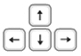
\includegraphics[height=20mm,width=20mm]{grafici/Tastisugiu.png}
 \vspace{-20pt}  
  %\caption{A gull}
\end{wrapfigure}

Possiamo scrivere diversi comandi prima di eseguirli (tasto di invio): basta separarli con un  ``;''.\\
Si ricordi sempre che \textsf{R} \`e {\emph case sensitive} ossia vi \`e differenza tra lettere minuscole e maiuscole.  Questo \`e particolarmente importante in quanto ad esempio le variabili \texttt{a} ed \texttt{A} rappresentano entit\`a distinte.
\subsection*{Editori esterni}
E' molto comodo scrivere le porzioni di codice che si intendono eseguire in \textsf{R} su un file di testo esterno in modo da disporre a fine sessione di un listato dei comandi usati (con eventuali commenti), scevro da errori e da operazioni superflue o ripetute.  Gli editor esterni hanno in particolare  la propriet\`a di
\begin{itemize}
\item Riconoscere la sintassi di \textsf{R} 
\item Interagire con \textsf{R}, consentendo l'esecuzione di comandi direttamente dall'editor. 
\end{itemize}
Ne menzioniamo quattro di semplice utilizzo: \textsf{Rstudio}, \textsf{Tinn-R}, \textsf{Komodo Edit} e \textsf{TextWrangler}, i cui dettagli sono presenti in tabella~\ref{editor}.\\
\begin{table}[htp]
\scriptsize
\begin{center}
\begin{tabular}{|c|c|c|}
\hline
Editor & Sistema Operativo & Website\\
\hline
\rst & Mutlipiattaforma & \url{http://www.Rstudio.org} \\
\textsf{Tinn-R} & Windows & \url{http://www.sciviews.org/Tinn-R} \\
\textsf{Komodo Edit} & Multipiattaforma & \url{http://www.activestate.com/komodo-edit}  \\
\textsf{TextWrangler} & Mac OSX & \url{http://www.barebones.com/products/textwrangler/}  \\ 
\hline
\end{tabular}
\end{center}
\caption{Alcune informazioni sugli editor citati nel testo (IDE)}
\label{editor}
\end{table}%
A parte \textsf{Tinn-R} e \rst, gli altri due editori necessitano di estensioni (\textit{plug-in}) dedicate per riconoscere la sintassi di \textsf{R}, segnalare errori, fornire suggerimenti ed eseguire comandi in \textsf{R} direttamente dall'editor. Il \textit{plug-in} per \textsf{Komodo Edit} si chiama \textsf{SciViews-K} (\url{http://www.sciviews.org}), mentre il \textit{plug-in} per \textsf{TextWrangler} \`e scaricabile dal sito \url{http://www.smalltime.com/gene/R.plist}. Quest'ultimo deve essere poi inserito nella directory (librerie globali): \texttt{\~{}/Library/Application Support/TextWrangler/Language Modules/}.\\
A livello di sviluppo sono invece disponibili editori dedicati, che forniscono numerose funzioni di diagnostica e \emph{debug} del codice. Senza qui addentrarci nei dettagli, \textsf{Emacs} (\url{http://www.gnu.org/software/emacs/}) con il \textit{plug-in} ESS (\textsf{Emacs} \textit{Speak Statistics}, \url{http://ess.r-project.org/}) ha trovato negli ultimi anni largo impiego anche come editor per \textsf{R}.
%%\footnote{per \textsf{Windows}, scaricabile  all'indirizzo \texttt{http://www.sciviews.org/Tinn-R/Tinn-R }}
%%, \footnote{Multipiattaforma, scaricabile all'indirizzo
%%\texttt{http://www.activestate.com/komodo-edit} che possiede estensioni per lavorare con  \textsf{R} scaricabili anche esse all'indirizzo \texttt{http://www.sciviews.org }}.
\\
Un discorso pi\`u esteso spetta ad \textsf{RStudio} che presenta un ambiente di sviluppo integrato particolarmente adatto a fini didattici e come  gi\`a detto \`e \emph{free} e multipiattaforma.  
\\
Adotteremo in questo libro \textsf{RStudio} per la facilit\`a d'uso e per il fatto che consente una visualizzazione completa contestuale di diversi aspetti di una sessione di lavoro. \textsf{RStudio} ha inoltre una versione server che  \`e stata resa disponibile all'indirizzo \url{http://rstudio.med.unipmn.it:8787/} per gli studenti di questo corso\footnote{Ringraziamo il Dottor Valter Rolando per essersi adoperato in tal senso}
%\begin{comment}
\section{Introduzione ad \textsf{Rstudio}}
All'apertura di \rst appaiono diversi pannelli mostrati in Figura~\ref{fig::Rstudiomain} 
  \begin{figure} 
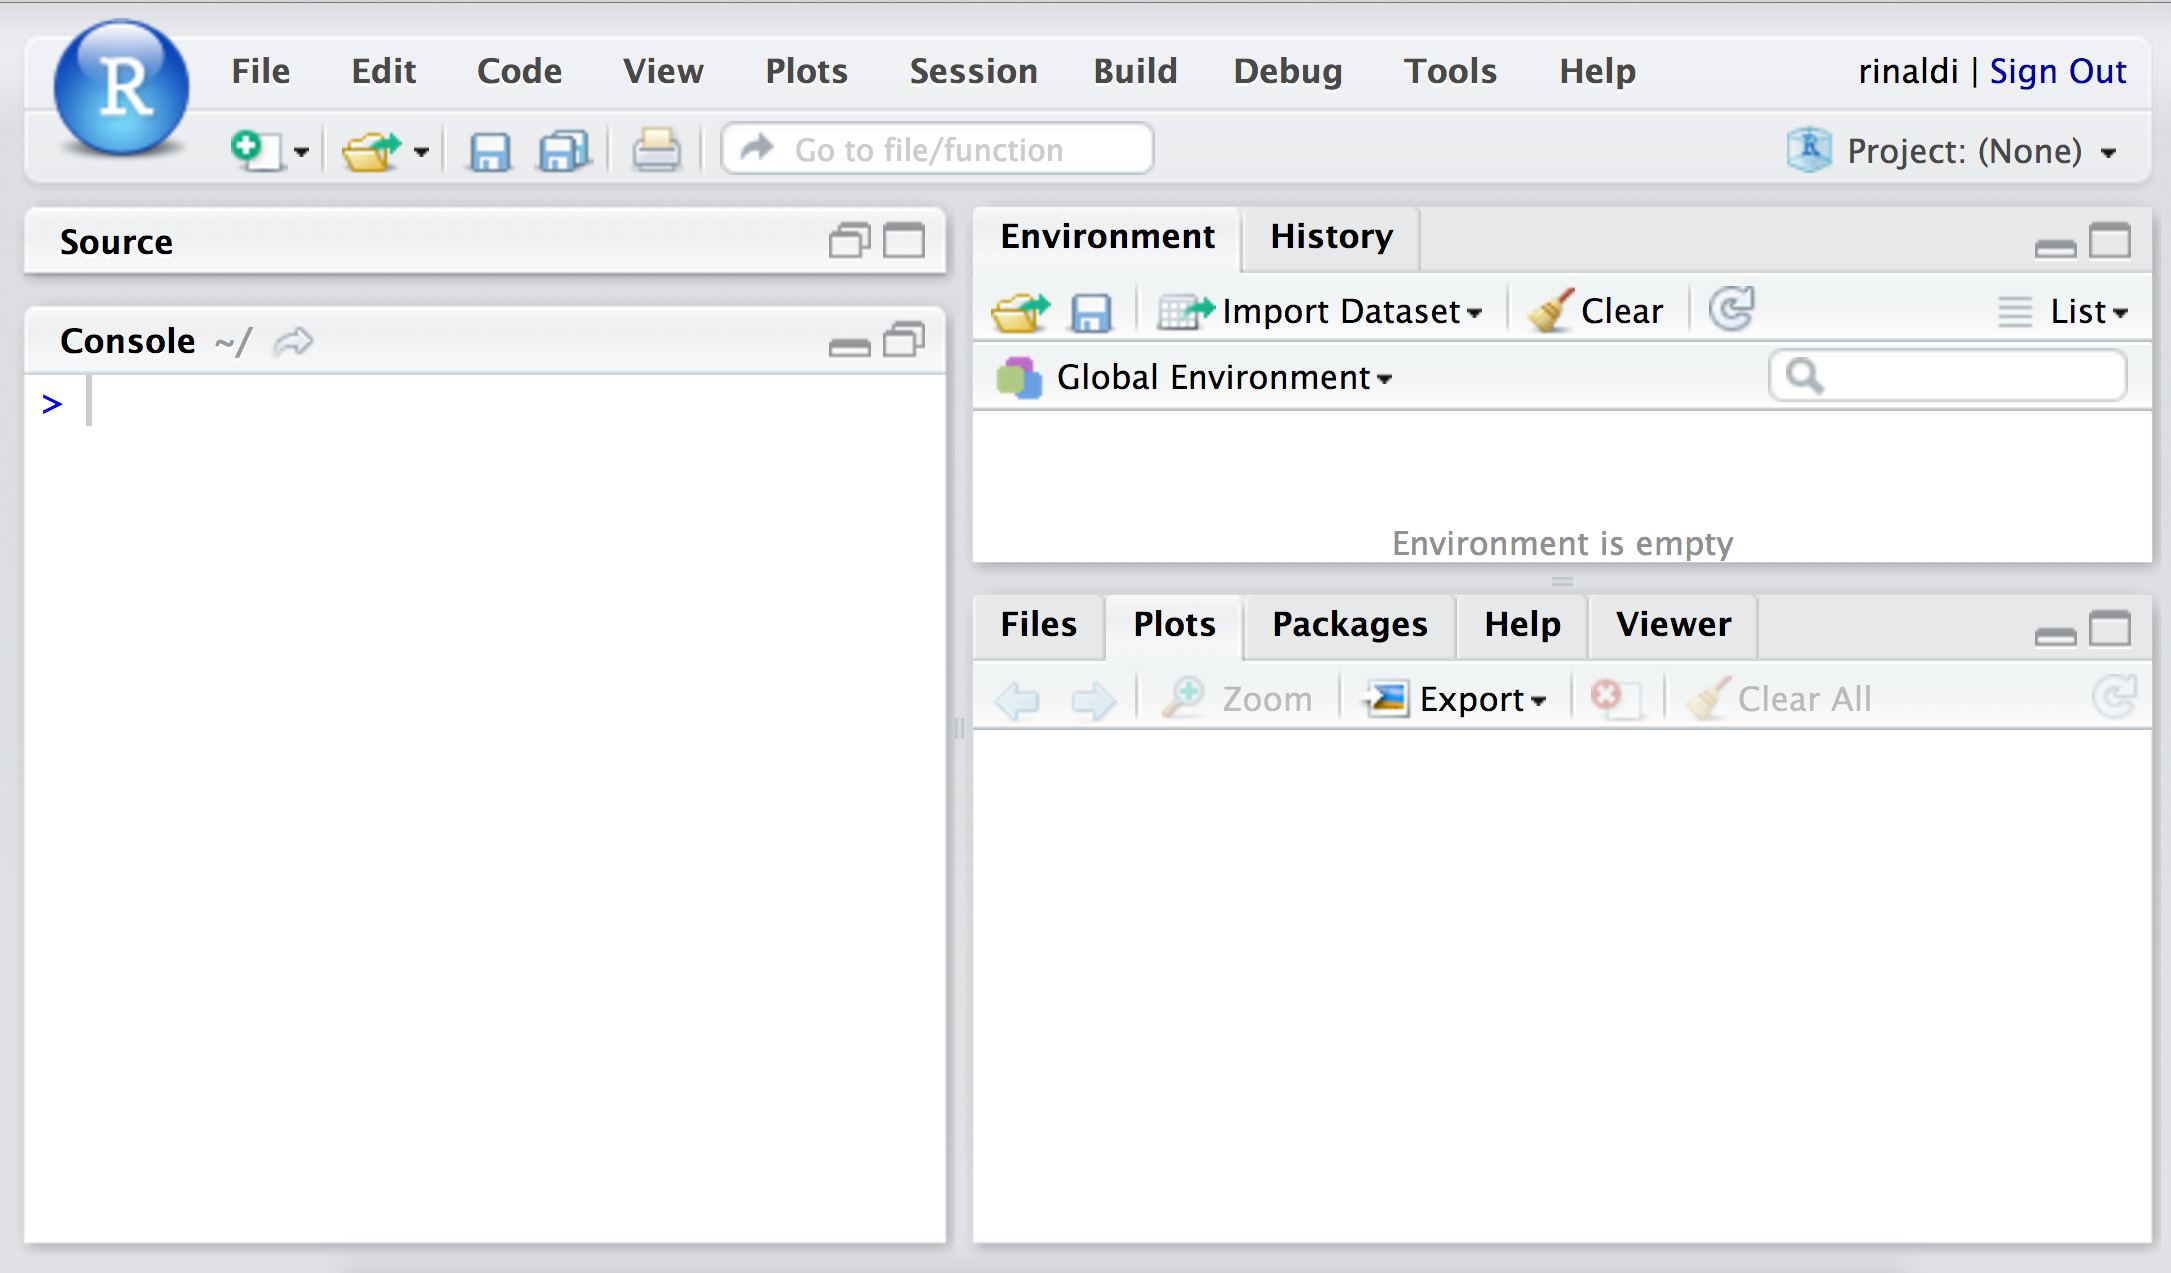
\includegraphics[width=1\textwidth]{grafici/Rstudiomain.png}
\caption{Finestra iniziale di  RStudio }
\label{fig::Rstudiomain} \end{figure}
 
Il pannello  fondamentale (a sinistra nella figura) \`e la classica console di \textsf{R}.
Ci sono poi 2 altri 2 pannelli a sinistra. Quello superiore   con 2 linguette  \texttt{Environment} e \texttt{History} e quello inferiore  con 5 linguette  \texttt{Files, Plots, Packages,Help, Viewer} il cui significato sar\`a presto chiarito.

La barra dei menu fornisce diversi menu a tendina che scopriremo procedendo nello studio.
 




\subsection*{Script di codice}
Dovendo scrivere porzioni di codice si pu\`o aprire un nuovo documento selezionando dal menu di \rpr in corrispondenza a \texttt{File} il tab \texttt{New Document} come in figura \ref{fig::Rscript}
 \begin{figure} [h]
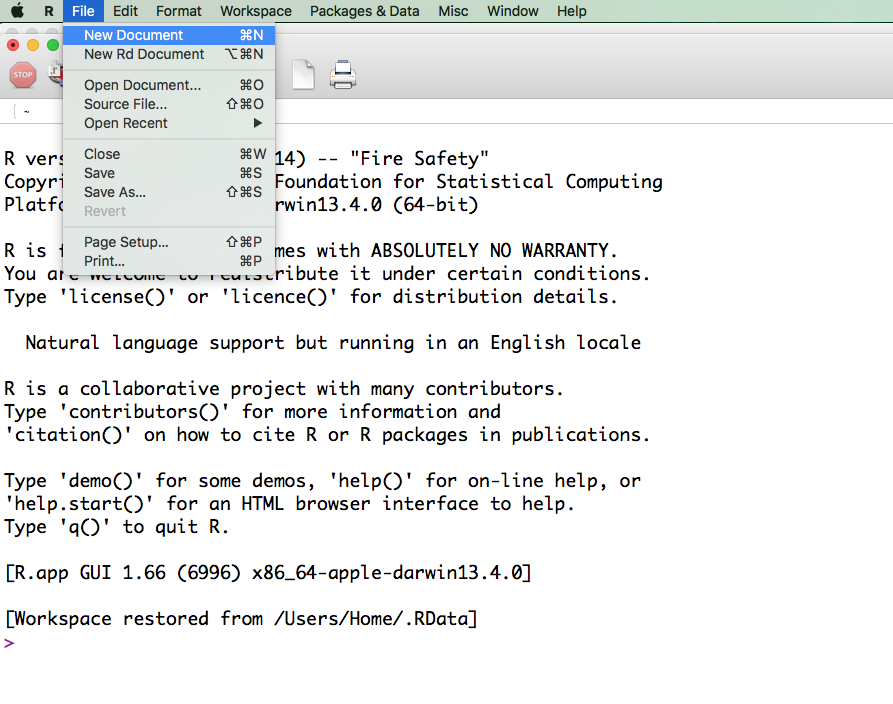
\includegraphics[width=1\textwidth]{grafici/newRdoc.png} 
\caption{Apertura  di uno script di \rpr in \rpr.}
\label{fig::Rscript} \end{figure}
\\
In \rst invece nel menu a relativo a \texttt{File}
si pu\`o selezionare \texttt{New file} e aprire file di diversa natura, in particolare porzioni di codice di \rst (R Script) come in figura~\ref{fig::Rstudioscript}.
Si provi per esempio ad aprire uno script di \rst e ad inserire il comando  
1+1.
\begin{figure} 
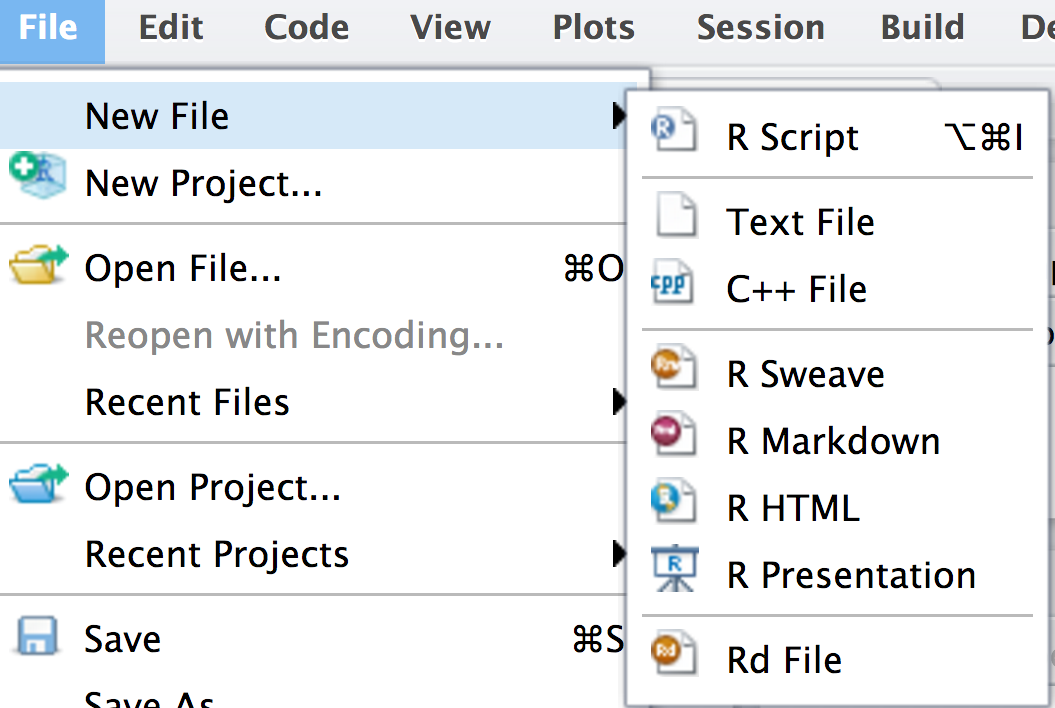
\includegraphics[width=0.4\textwidth]{grafici/Rscript.png}\hskip40pt
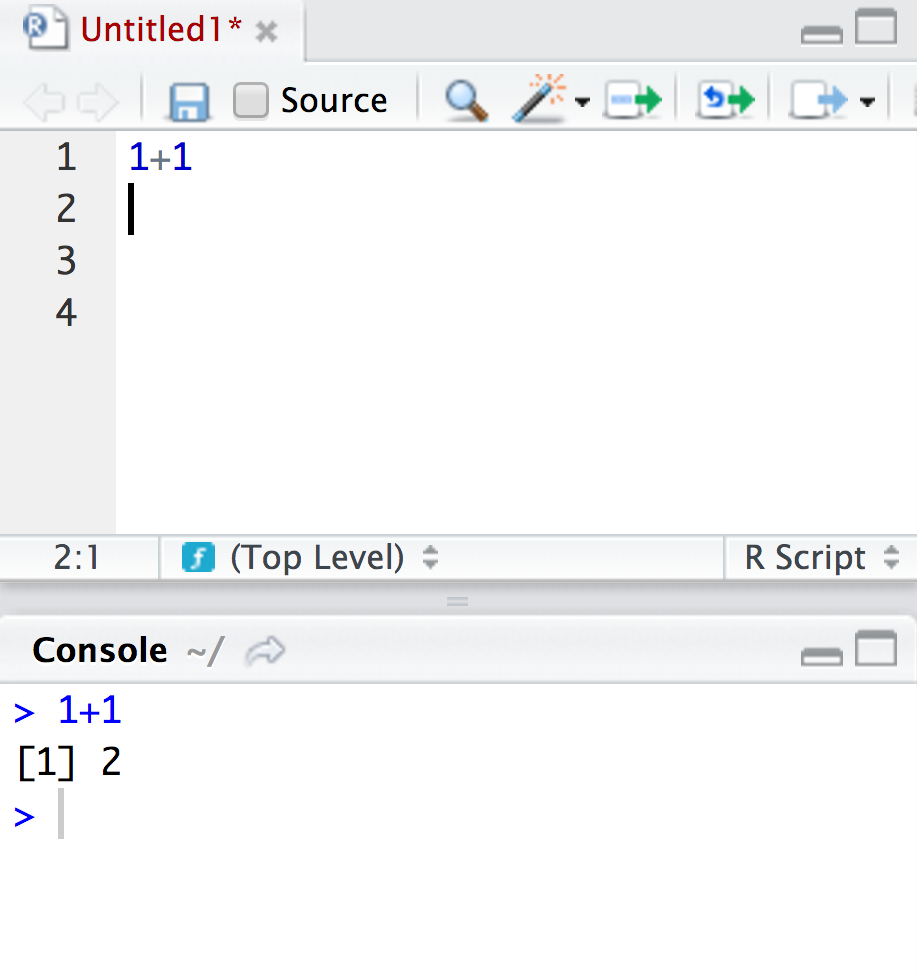
\includegraphics[width=0.4\textwidth]{grafici/esecuzione.png}
\caption{Apertura  ed esecuzione di uno script di \rpr in  \rst }
\label{fig::Rstudioscript} \end{figure}

Usando le frecce o le scorciatoie da tastiera nel menu a tendina in corrispondenza a \texttt{code} si possono inviare i comandi a \rpr per la loro esecuzione.
 

Il file va poi salvato in una cartella opportuna  con estensione \texttt{.R}.

 \subsection*{Help e guida on-line}
Una qualunque richiesta di informazioni pu\`o essere effettuata digitando il comando:
$?\varia{argomento}$   (o $\texttt{help}(\varia{argomento}))$.
\index{\texttt{help}} 
Ad esempio $?\texttt{sin}$  consente di ottenere informazioni sulla funzione seno e altre funzioni trigonometriche in quanto la guida \`e completamente indicizzata. \`E anche possibile utilizzare il menu a tendina ({\it help}), con modalit\`a diverse a seconda del sistema operativo.\\
%Infine, il comando \texttt{help.start()} consente di aprire l'\textit{help} HTML di \textsf{R} da cui \`e poi possibile consultare %la documentazione.
In RStudio basta invece clicare sul menu Help selezionare la casellina Home e scrivere il comando al quale si \`e interessati.
\subsection*{Inserire i commenti}  
I commenti sono frasi, annotazioni o codice da non eseguire momentaneamente molto utilizzati in programmazione. L'introduzione di un commento in \textsf{R} \`e possibile mediante il simbolo \texttt{\#} (cancelletto singolo o \emph{hash}). Per evitare che un commento venga cancellato durante il normale \textit{editing} del testo e che esso venga eseguito si consiglia di raddoppiare i simboli (\texttt{\#\#}). Ad esempio:
\index{\texttt{\#}} 
\begin{Schunk}
\begin{Sinput}
> 1+1 # dovrebbe fare 2
\end{Sinput}
\begin{Soutput}
[1] 2
\end{Soutput}
\end{Schunk}
non produrr\`a errore perch\'e riconoscer\`a la stringa scritta dopo \texttt{\#} come commento.

\subsubsection{Quando un commento \`e utile e quando \`e superfluo?}
A prescindere dalle preferenze personali, un commento dovrebbe essere inserito quando la porzione di codice che si sta considerando risulta a noi non ovvia, quando le dimensioni, tipo e ruolo delle variabili coinvolte non sono ovvie o semplicemente quando si ha bisogno di introdurre una annotazione che renda pi\`u facile la lettura del codice non solo a noi stessi ma anche ad altri. Quest'ultimo punto \`e di fondamentale importanza quando si vuole condividere il codice con altri membri della comunit\`a scientifica. Per capire se i commenti che inserite sono superflui o mancanti:
\begin{shaded}
Ad un certo punto del corso salvate una porzione di codice (o una funzione) commentata in un file \texttt{.R}, lunga almeno 25 righe di codice. Aggiungete la data corrente al nome del file e in un periodo compreso tra 6 e 12 mesi semplicemente aprite il file e rileggetene il codice. Se siete in grado di capirne il contenuto, avete probabilmente fatto buon uso dei commenti.
 \end{shaded} 

\subsection*{Working directory}
Il comando \index{\texttt{getwd()}} 
%codechunk
\begin{Schunk}
\begin{Sinput}
> getwd()
\end{Sinput}
\end{Schunk}
indica la directory di lavoro mentre il comando 
%codechunk
\begin{Schunk}
\begin{Sinput}
> setwd("indirizzo")
\end{Sinput}
\end{Schunk}
\index{\texttt{setwd()}} 
 imposta la {\it working directory}  nella posizione specificata da \texttt{"indirizzo"}. 
 Lavorando con \rst per impostare la directory si pu\`o usare il menu a tendina
\texttt{Session};  \`e  in particolare  possibile posizionare la \texttt{working directory} in corrispondenza al file di codice sorgente (\texttt{To Source File location}). 


\subsection*{Pacchetti}

Oltre all'aggiornamento costante del programma, lo sviluppo di \rpr consiste nello creazione e aggiornamento continui da parte della comunit\`a  mondiale di una serie di pacchetti addizionali. Un pacchetto contiene in particolare un insieme di comandi finalizzati alla  realizzazione di un determinato compito: esistono per esempio pacchetti per la risoluzione di equazioni differenziali, pacchetti per l'analisi statistica di {\it microarray}, pacchetti per il {\it clustering} di dati.  Per non appesantire \rpr i pacchetti (con poche eccezioni) vengono caricati solo se richiesto dalle esigenze dell'utente. 
L'utente deve quindi inizialmente localizzare (per esempio via web) il pacchetto che lo interessa e scaricarlo localmente.  
Per fare questo deve selezionare il sito CRAN da cui scaricarlo e poi (direttamente dal menu a tendina di \rpr) scaricarlo (con annesse eventuali {\it dependencies}). Una volta scaricato in locale il pacchetto pu\`o essere messo a disposizione dell'utente con il comando  
%codechunk
\begin{Schunk}
\begin{Sinput}
> library("nome.pacchetto")
\end{Sinput}
\end{Schunk}

Se si lavora all'interno di \rst il caricamento dei pacchetti \`e pi\`u semplice: in uno dei pannelli \`e presente il menu \texttt{Packages} dal quale l'utente pu\`o scaricare il pacchetto usando il sottomenu \texttt{Install} e caricarlo all'interno di \rpr semplicemente barrandone la casellina relativa.

\chapter{Introduzione ad \rpr}

\section{Variabili}
Una variabile \`e una porzione di memoria caratterizzata da un nome che contiene dati che possono essere modificati durante l'esecuzione del programma.\\ \`E  possibile definire una qualunque variabile mediante l'assegnazione di un valore ad essa.\\
Sono valide entrambe le notazioni seguenti:
$ \varia{variabile}\leftarrow\varia{ valore}$ e
$\varia{valore} \to  \varia{variabile}$;
ad esempio:
\begin{Schunk}
\begin{Sinput}
> a<-2 
\end{Sinput}
\end{Schunk}
associa il valore $2$ alla variabile \texttt{a}. Per comporre le frecce si usano i segni ``meno'' ``maggiore''  \texttt{->}(freccia a destra) o ``minore'' ``meno''  \texttt{<-}(freccia a sinistra).
Si abbia cura di evitare di inserire spazi tra il nome della variabile e la freccia, cos\`\i \; come tra la freccia ed il valore assegnato. Il programma per assegnazioni semplici non invia  alcun messaggio di errore, ma si possono verificare problemi quando vi siano pi\`u membri costituenti il valore assegnato.
Rivolgere {\bf sempre} la freccia dal valore alla variabile, infatti essa \`e una scatola in grado di contenere il valore voluto. Ad esempio non \`e valida la stringa:
$variabile\rightarrow valore $ o $ valore\leftarrow variabile$.
{\bf Non} lasciare spazi vuoti nel definire il nome della variabile, \`e possibile invece utilizzare  il sottotratto (\textit{underscore}) $\_$  ad esempio definendo: \texttt{variabile\_uno}, {\bf non} \texttt{variabile uno}. Si pu\`o anche usare il punto e scrivere  \texttt{variabile.uno}.
I nomi delle variabili sottostanno ad alcune regole. Per esempio \texttt{variabile1} \`e un nome lecito mentre non lo \`e  \texttt{1variabile}.\\  L'assegnamento di uno stesso valore a pi\`u variabili (o costanti) in un unico comando \`e possibile con una sintassi del tipo: 
\begin{Schunk}
\begin{Sinput}
> a<-b<-c<-5 
\end{Sinput}
\end{Schunk}
L'assegnazione pu\`o avvenire anche usando il segno `$=$', ad esempio
\begin{Schunk}
\begin{Sinput}
> a=5 
\end{Sinput}
\end{Schunk}
o il comando
\begin{Schunk}
\begin{Sinput}
> assign("a",5)
\end{Sinput}
\end{Schunk}
Ogni variabile \`e richiamabile scrivendo il suo nome.
Ad esempio:
\texttt{a} richiama la variabile \texttt{a} appena definita e mostra il valore di \texttt{a} in output, ovvero 5\footnote{Spesso 
dopo aver scritto un comando ad esempio \texttt{a<-5} ci si interroga sull'assenza di output. In realt\`a il comando \`e stato eseguito. Per verificarlo basta scrivere \texttt{a} ed inviare. In modo alternativo il comando  \texttt{(a<-5)} oltre a definire l'associazione di 5 ad \texttt{a} ne stampa il valore.},
Per rimuovere una variabile o un generico oggetto si utilizza il comando:
$$\texttt{rm}(\varia{name}),$$
 ossia {\it remove memory}, \varia{name} \`e il nome della variabile da cancellare. Ad \index{\texttt{rm()}} esempio: 
\begin{Schunk}
\begin{Sinput}
> rm(a)
> a=5;a
\end{Sinput}
\begin{Soutput}
[1] 5
\end{Soutput}
\end{Schunk}
svuota il contenuto della memoria \texttt{a}. Per conoscere gli oggetti presenti nella sessione corrente basta il comando
\begin{Schunk}
\begin{Sinput}
> ls()
\end{Sinput}
\begin{Soutput}
[1] "a" "b" "c"
\end{Soutput}
\end{Schunk}
o in modo equivalente
\begin{Schunk}
\begin{Sinput}
> objects()
\end{Sinput}
\begin{Soutput}
[1] "a" "b" "c"
\end{Soutput}
\end{Schunk}
L'insieme degli oggetti presenti in una sessione costituisce il \textsl{worksapce} o \textsl{environment} (ambiente di lavoro) il cui contenuto \`e facilmente visualizzabile in \rst   cliccando su \texttt{Environment}.
Scoprire come eliminare gli oggetti. 

\section{Costruzione di vettori}  Un vettore (o \textit{array} monodimensionale) 
pu\`o essere visto come un casellario, le cui caselle sono dette celle (\emph{slot}) del vettore stesso. Tutte le celle sono variabili di uno stesso tipo, detto tipo base del vettore. Si possono cos\`\i\  definire vettori di numeri, di caratteri e vettori logici. 
%In alcuni linguaggi una stringa \`e vista come un vettore di caratteri. 
%Spesso inoltre la dimensione di un vettore (il numero celle di cui esso \`e composto) viene considerato parte della definizione,
In \textsf{R} l'assegnamento della dimensione di un vettore non \`e obbligatorio. %Nel testo ci riferiremo ad un vettore utilizzando anche il termine elenco, che per comodit\`a consideriamo analogo. 
Un vettore pu\`o  essere definito utilizzando il comando \texttt{c} di sintassi generale:  
\index{\texttt{c}}
\begin{equation*}
\texttt{c}(\varia{valore}_1, \varia{valore}_2, \ldots,\varia{valore}_n)
\end{equation*}
Ad esempio
\begin{Schunk}
\begin{Sinput}
>  c(1,5,9,11,17,34)
\end{Sinput}
\begin{Soutput}
[1]  1  5  9 11 17 34
\end{Soutput}
\end{Schunk}
Si pu\`o associare il vettore ad una variabile con la notazione:
\begin{equation*}
\texttt{c}(\varia{valore}_1, \varia{valore}_2, \varia{valore}_n)\rightarrow \varia{variabile}
\end{equation*}
Per esempio:
\begin{Schunk}
\begin{Sinput}
> c(1,5,9,11,17,34)->vettore
\end{Sinput}
\end{Schunk}
Due operazioni fondamentali sono l'estrazione di una cella
\begin{Schunk}
\begin{Sinput}
> i=4;vettore[i]
\end{Sinput}
\begin{Soutput}
[1] 11
\end{Soutput}
\end{Schunk}
e la sostituzione
\begin{Schunk}
\begin{Sinput}
> vettore[i]<-5
\end{Sinput}
\end{Schunk}
Si noti anche che se scriviamo
\begin{Schunk}
\begin{Sinput}
> vettore[i]<-"testo"
> vettore
\end{Sinput}
\begin{Soutput}
[1] "1"     "5"     "9"     "testo" "17"    "34"   
\end{Soutput}
\end{Schunk}
abbiamo anche cambiato il tipo di base del vettore mentre, se scriviamo
\begin{Schunk}
\begin{Sinput}
> vettore[i]<-11
> vettore
\end{Sinput}
\begin{Soutput}
[1] "1"  "5"  "9"  "11" "17" "34"
\end{Soutput}
\end{Schunk}
il vettore non viene restaurato. Per farlo occorre in questo caso scrivere
\begin{Schunk}
\begin{Sinput}
> as.numeric(vettore)->vettore 
\end{Sinput}
\end{Schunk}
Possiamo anche definire celle con indice superiore alla lunghezza
\begin{Schunk}
\begin{Sinput}
> vettore[10]<-3
> vettore
\end{Sinput}
\begin{Soutput}
 [1]  1  5  9 11 17 34 NA NA NA  3
\end{Soutput}
\end{Schunk}
 il vettore viene prolungato fino a comprendere 10 celle. Le celle non assegnate vengono etichettate con \texttt{NA} (not assigned).
 Se invece si scrive
\begin{Schunk}
\begin{Sinput}
> vettore[-3]
\end{Sinput}
\begin{Soutput}
[1]  1  5 11 17 34 NA NA NA  3
\end{Soutput}
\end{Schunk}
la cella di posizione 3 viene eliminata.
Possiamo determinare la lunghezza di un vettore con la funzione \texttt{length}:
\index{\texttt{length}}
\begin{Schunk}
\begin{Sinput}
> length(vettore)
\end{Sinput}
\begin{Soutput}
[1] 10
\end{Soutput}
\end{Schunk}
 Possiamo poi ovviamente eseguire operazioni sui vettori
\begin{Schunk}
\begin{Sinput}
> 3*vettore
\end{Sinput}
\begin{Soutput}
 [1]   3  15  27  33  51 102  NA  NA  NA   9
\end{Soutput}
\end{Schunk}
 
Il vettore di nome \texttt{vettore}, viene moltiplicato per 3, ovvero ciascuna cella viene moltiplicata per 3.
\subsection{Generazione di sequenze: $\texttt{rep}$ e $\texttt{seq}$} 
\`E possibile definire sequenze di numeri consecutivi come  \varia{n:m}.
Ad esempio:
\begin{Schunk}
\begin{Sinput}
> 1:11 
\end{Sinput}
\begin{Soutput}
 [1]  1  2  3  4  5  6  7  8  9 10 11
\end{Soutput}
\end{Schunk}
consente di ottenere la sequenza dei numeri interi da 1 a 11. \`E anche possibile aggiungere un numero alla sequenza con il comando: 
$\texttt{c}(\varia{n:m},\varia{numero \; aggiunto})$.
Per esempio se vogliamo aggiungere il numero 100 alla lista precedente scriveremo:
\begin{Schunk}
\begin{Sinput}
> c(1:11,100)
\end{Sinput}
\begin{Soutput}
 [1]   1   2   3   4   5   6   7   8   9  10  11 100
\end{Soutput}
\end{Schunk}
Nota: l'aggiunta \`e posizionale, cio\`e rispetta l'ordine con cui compaiono gli elementi. 

\`E inoltre possibile generare liste costanti di valore $k$ con il comando:
$\texttt{rep} (\varia{k,n})$
Se vogliamo una lista i cui elementi sono tutti 3 per un totale di 10 elementi scriveremo:
\begin{Schunk}
\begin{Sinput}
> rep(3,10)
\end{Sinput}
\begin{Soutput}
 [1] 3 3 3 3 3 3 3 3 3 3
\end{Soutput}
\end{Schunk}
Infine il parametro \texttt{each=}\varia{n} consente di ripetere ciascun elemento della sequenza \varia{n} volte. Ad esempio:
\begin{Schunk}
\begin{Sinput}
> rep(c(3,2,1),each=3)
\end{Sinput}
\begin{Soutput}
[1] 3 3 3 2 2 2 1 1 1
\end{Soutput}
\end{Schunk}
Ripete 3 volte il numero 3, 3 volte il numero 2 e 3 volte il numero 1. 
Diverso \`e il risultato con il comando 
\begin{Schunk}
\begin{Sinput}
> rep(c(3,2,1),times=5)
\end{Sinput}
\begin{Soutput}
 [1] 3 2 1 3 2 1 3 2 1 3 2 1 3 2 1
\end{Soutput}
\end{Schunk}
dove si ha la ripetizione \texttt{times} volte dell'intero vettore.
Cosa succede se 2 vettori hanno lunghezza diversa? In matematica tradizionalmente questa somma non \`e definita. In \rpr invece vale la regola del riciclaggio  (\textit{recycling rule}). Se dobbiamo sommare i vettori che seguono 
 \begin{align*} &(1,2,3,4,5,6,7,8)+\\ &(3,4,5)\hskip50pt =\\
 &\noindent\rule{0.25\textwidth}{0.4pt}\\
\end{align*} 
si procede cos\'\i: la somma
si calcola riciclando il vettore pi\`u breve
 \begin{align} 
&(1,~2,~3,~4,~5,~6,~7,~8)+\\
&(3,~4,~5,~3,~4,~5,~3,~4)=\\
&\noindent\rule{0.3\textwidth}{0.8pt} \\
&(4, ~ 6,~  8 ,~ 7,~  9 ,11, 10,12)\\
\end{align}
In modo simile se dobbiamo sommare i vettori che seguono 
 \begin{align*} &(1,2,3,4,5,6,7,8)+\\ &(3)\hskip70pt =\\
 &\noindent\rule{0.3\textwidth}{0.6pt}\\
\end{align*} 
si esegue la somma
\begin{align} 
&(1,~2,~3,~4,~5,~6,~7,~8)+\\
&(3,~3,~3,~3,~3,~3,~3,~3)=\\
&\noindent\rule{0.3\textwidth}{0.8pt} \\
&(4, ~ 5,~  6 ,~ 7,~  8 ,~9, 10,11)\\
\end{align} 
Ad esempio
\begin{Schunk}
\begin{Sinput}
> 1:8+3:5
\end{Sinput}
\begin{Soutput}
[1]  4  6  8  7  9 11 10 12
\end{Soutput}
\begin{Sinput}
> 1:8+3
\end{Sinput}
\begin{Soutput}
[1]  4  5  6  7  8  9 10 11
\end{Soutput}
\end{Schunk}
In pratica il vettore pi\`u corto viene riciclato tante volte quanto serve per raggiungere la lunghezza del vettore pi\`u lungo. Se la ripetizione non occorre un numero intero di volte allora viene emesso un messaggio di \textit{Warning}.

Il comando \texttt{seq} consente di generare una sequenza (vettore) i cui elementi sono collegati da una propriet\`a caratteristica: sono tutti numeri pari, dispari, di passo $n$, ecc.\\
Si definisce una sequenza come: $\texttt{seq}(\varia{n,m})$\\ %%
Ad esempio per generare la sequenza dei numeri da 0 a 100 a passo 1 (default) si scriver\`a:
\index{\texttt{seq}}
\begin{Schunk}
\begin{Sinput}
> seq(0,100,1) ##analogo di seq(0,100)
\end{Sinput}
\begin{Soutput}
  [1]   0   1   2   3   4   5   6   7   8   9  10  11  12
 [14]  13  14  15  16  17  18  19  20  21  22  23  24  25
 [27]  26  27  28  29  30  31  32  33  34  35  36  37  38
 [40]  39  40  41  42  43  44  45  46  47  48  49  50  51
 [53]  52  53  54  55  56  57  58  59  60  61  62  63  64
 [66]  65  66  67  68  69  70  71  72  73  74  75  76  77
 [79]  78  79  80  81  82  83  84  85  86  87  88  89  90
 [92]  91  92  93  94  95  96  97  98  99 100
\end{Soutput}
\end{Schunk}
Possiamo ottenere la sequenza di tutti i numeri dispari da $n$ a $m$ utilizzando il parametro \texttt{by},che consente di impostare il passo nella sequenza.
Il comando:  
\begin{Schunk}
\begin{Sinput}
> seq(1,100,by=2)
\end{Sinput}
\begin{Soutput}
 [1]  1  3  5  7  9 11 13 15 17 19 21 23 25 27 29 31 33 35
[19] 37 39 41 43 45 47 49 51 53 55 57 59 61 63 65 67 69 71
[37] 73 75 77 79 81 83 85 87 89 91 93 95 97 99
\end{Soutput}
\end{Schunk}
restituisce tutti i numeri tra 1 e 100 a passo 2, ovvero tutti i numeri dispari compresi nell'intervallo. 
Per ottenere i numeri pari compresi nell'intervallo possiamo reiterare il comando precedente ma partendo da 0 (e volendo possiamo sottintendere la specifica \texttt{by=})
\begin{Schunk}
\begin{Sinput}
> seq(0,100,2)
\end{Sinput}
\begin{Soutput}
 [1]   0   2   4   6   8  10  12  14  16  18  20  22  24  26
[15]  28  30  32  34  36  38  40  42  44  46  48  50  52  54
[29]  56  58  60  62  64  66  68  70  72  74  76  78  80  82
[43]  84  86  88  90  92  94  96  98 100
\end{Soutput}
\end{Schunk}
il parametro \texttt{length.out}  (brevemente \texttt{len} o \texttt{length} consente di definire il numero totale di elementi della sequenza, ovvero divide l'intervallo  da $m$ a $n$ utilizzando un numero di punti pari alla lunghezza assegnata.
Ad esempio se nella  sequenza di numeri da 1 a 100 volessimo avere in totale 10 numeri scriveremo: 
\begin{Schunk}
\begin{Sinput}
> seq(1,100,length=10)
\end{Sinput}
\begin{Soutput}
 [1]   1  12  23  34  45  56  67  78  89 100
\end{Soutput}
\end{Schunk}
In effetti l'intevallo da 1 a 100  di lunghezza 99 viene diviso da 10 punti in 9 parti di ampiezza 11. Useremo tale parametro per il calcolo degli integrali con il metodo dei rettangoli.\\
  \begin{shaded}
  \begin{description}
\item{1.} Costruire un vettore contenente i numeri da 1 a 15. Identificare almeno due modi per invertire l'ordine degli elementi. Scambiare poi  il $5^o$  e il $6^o$ ingresso del vettore e stampare a video il risultato.
\item{2.} Calcolare $23+37/10-2^3$
\item{3.} Scrivere il vettore 
$x =(1,1,2,3,5,8)$.
Stampare il $3^o$  elemento di $x$. Determinare la lunghezza di $x$. 
Costruire un vettore i cui elementi siano la radice quadrata degli elementi di $x$.
\item{4.} Si consideri la funzione $f(x)=x*\sin(x)$. Si determinino i valori di $f$ negli estremi della suddivisione dell'intervallo $[2,5]$  in 20 sotto-intervalli di ugual ampiezza.
\end{description}
\end{shaded}
\chapter{Matematica di Base}
In quanto segue immaginiamo di operare direttamente in \rpr anche se avere a disposizione il listato dei comandi pu\`o essere utile.
\section{Numeri, operazioni aritmetiche e variabili}
\subsection{I numeri}
Se scriviamo in \rpr qualunque numero la rappresentazione che ne abbiamo \`e quella di un numero reale dove  il punto viene usato come separatore decimale. Inoltre per numeri molto grandi o molto piccoli \rpr ricorre alla notazione scientifica. Un numero  ``grande''  viene scritto come
\varia{ae + b} (senza spazi) mentre un numero  ``piccolo'' viene scritto come
\varia{ae - b} (senza spazi) 
dove $a$ varia tra 1 e 9 e $b$  \`e l'esponente opportuno (in base 10). Ad esempio:
\begin{Schunk}
\begin{Sinput}
> 0.0001
\end{Sinput}
\begin{Soutput}
[1] 1e-04
\end{Soutput}
\begin{Sinput}
> 5.4e6
\end{Sinput}
\begin{Soutput}
[1] 5400000
\end{Soutput}
\end{Schunk}
Si abbia cura di utilizzare il punto `.' invece della virgola `,'  come separatore decimale.  Il comando \texttt{class()} fornisce la natura di un oggetto.

Per quanto riguarda le operazioni aritmetiche fondamentali si usano i simboli:
`$+$', `$-$',`$*$' e~`$/$'. Per l'elevamento a potenza il simbolo  \`e `\texttt{\^}'.

Si noti  che il numero di cifre di cui \textsf{R} dispone  \`e superiore al numero di cifre visualizzate
\begin{Schunk}
\begin{Sinput}
> a=4/3
> a
\end{Sinput}
\begin{Soutput}
[1] 1.333333
\end{Soutput}
\begin{Sinput}
> a*3
\end{Sinput}
\begin{Soutput}
[1] 4
\end{Soutput}
\begin{Sinput}
> 1.333333*3
\end{Sinput}
\begin{Soutput}
[1] 3.999999
\end{Soutput}
\end{Schunk}



\subsection{Costanti fondamentali}
Per costante ci si riferisce ad un valore non modificabile. Ogni linguaggio permette di utilizzare diversi tipi di costanti: numeri, caratteri e stringhe.\\  Tra le costanti definite in \rpr~di interesse generale abbiamo
\index{\texttt{pi}}
\begin{itemize}
\item{}$\pi$ definito come \texttt{pi}.
\item{}\texttt{e}: numero di Nepero 
definito come il  valore  in $x=1$ della funzione esponenziale \texttt{exp(1)}. La notazione \`e equivalente ad $e^1$.
Non \`e possibile definire \texttt{e} solo con la stringa \texttt{exp} senza assegnare l'esponente, in quanto esso \`e definito come una funzione di $x$.  
Ovviamente le costanti sono utilizzabili in qualsiasi calcolo:
\begin{Schunk}
\begin{Sinput}
> duepi<-2*pi
> duepi
\end{Sinput}
\begin{Soutput}
[1] 6.283185
\end{Soutput}
\end{Schunk}
Abbiamo assegnato alla variabile \texttt{duepi}  valore $2*\pi$  e l'abbiamo richiamata per visualizzare il risultato.\\
Nota bene: se si intende visualizzare il valore e non ad utilizzarlo in calcoli successivi \`e pi\`u comodo ricorrere alla visualizzazione a \emph{console}, come nell'esempio:
\begin{Schunk}
\begin{Sinput}
> 2*pi
\end{Sinput}
\begin{Soutput}
[1] 6.283185
\end{Soutput}
\end{Schunk}
in output si ottiene direttamente il risultato del calcolo.  
\end{itemize}
 

 
\subsection{Interi e frazioni}
Se scriviamo
\begin{Schunk}
\begin{Sinput}
> class(5)
\end{Sinput}
\begin{Soutput}
[1] "numeric"
\end{Soutput}
\end{Schunk}
notiamo che il numero intero 5 \`e stato interpretato come un numero reale.
Se desideriamo espressamente ricordarci che  5 \`e  un  intero possiamo scrivere 5L
\begin{Schunk}
\begin{Sinput}
> class(5L)
\end{Sinput}
\begin{Soutput}
[1] "integer"
\end{Soutput}
\end{Schunk}
Possiamo inoltre lavorare con le frazioni caricando il pacchetto \texttt{MASS} e usando la sintassi
\texttt{fractions(m/n)}
\begin{Schunk}
\begin{Sinput}
> library(MASS)
> fractions(1/4)+fractions(2/3)
\end{Sinput}
\begin{Soutput}
[1] 11/12
\end{Soutput}
\end{Schunk}



\begin{itemize}
\begin{question}
Si calcoli la frazione
17/5+20/7
\end{question}

\begin{solution}
Si determina il denominatore comune prendendo il minimo comune multiplo di 5 e 7.
\end{solution}
\begin{question}
Si calcoli la frazione
1/2+7/8
\end{question}
\\
\begin{question}
2/5+6/5
\end{question}

\end{itemize}
\begin{comment}\subsection{Equazioni lineari}
%Consideriamo semplici equazioni lineari del tipo
$$ a x +b =cx+d$$
Per risolvere si portano i termini con la variabile $x$ da una parte e i termini noti dall'altra
$$(a-c) x=d-b$$
e la soluzione unica \`e  (se $a-c$ \`e diverso da 0)
$x=\dfrac{d-b}{a-c}$.
In \rpr  per risolvere 
$$ 10 x+ 5=2 x+7$$
basta scrivere
\begin{Schunk}
\begin{Sinput}
> a=10
> b=5
> c=2
> d=7
> solve(a-c,d-b)
\end{Sinput}
\begin{Soutput}
[1] 0.25
\end{Soutput}
\end{Schunk}
Tale comando non \`e qui particolarmente conveniente ma vedremo che si generalizza alla risoluzione di sistemi lineari.
\end{comment}
\section{Funzioni e grafici}
\subsection{Definizione di funzioni}
Per definire una funzione $f$ di una variabile \varia{variabile}  si utilizza il comando:
$$f\leftarrow \texttt{function}(\varia{variabile})\; \varia{espressione}$$
Ad esempio per definire la funzione $$f(x)=x^2$$ scriveremo:  
\begin{Schunk}
\begin{Sinput}
> f<-function(x) x^2
\end{Sinput}
\end{Schunk}
Possiamo calcolare il valore della funzione in un qualunque valore di $x$  con il comando:
\texttt{f}(\varia{valore})
ad esempio in $x=6$ si avr\`a 
\begin{Schunk}
\begin{Sinput}
> f(6)
\end{Sinput}
\begin{Soutput}
[1] 36
\end{Soutput}
\end{Schunk}
Attenzione: nell'esempio che segue viene richiesto il valore di $f(x)$ in $x=0$:
\begin{Schunk}
\begin{Sinput}
> f<-function(x)  1/x 
> f(0)
\end{Sinput}
\begin{Soutput}
[1] Inf
\end{Soutput}
\end{Schunk}
La dicitura \texttt{Inf} corrisponde ad $\infty$, infatti la funzione esplode in $x=0$.


\subsection{Funzioni predefinite}  
\rpr consente l'utilizzo di funzioni matematiche gi\`a definite, come seno, coseno, tangente, le funzioni trigonometriche inverse, esponenziali, logaritmi, radici,ecc.
Ecco di seguito le principali, la cui sintassi pu\`o essere visualizzata utilizzando l'\emph {help} di \rpr inserendo la parola chiave corretta (ad esempio \texttt{?sin}) per ottenere informazioni sul formalismo corretto:  
\begin{itemize}
 \item{}
 Funzioni trigonometriche\hfill\vskip10pt
 \begin{tabular}{|r r |}\hline
\texttt{cos}&  coseno\\
\texttt{sin}& seno\\
\texttt{tan}&   tangente\\
\texttt{acos}&   arcocoseno\\
\texttt{asin}&   arcoseno\\
\texttt{atan} &  arcotangente\\
\hline
\end{tabular}
\item{}Logaritmi.\vskip10pt
\texttt{log} \`e il  logaritmo naturale. Ad esempio:
\begin{Schunk}
\begin{Sinput}
> log(3)
\end{Sinput}
\begin{Soutput}
[1] 1.098612
\end{Soutput}
\end{Schunk}
\texttt{log2} \`e il logaritmo di base 2 
\begin{Schunk}
\begin{Sinput}
> log2(3)
\end{Sinput}
\begin{Soutput}
[1] 1.584963
\end{Soutput}
\end{Schunk}
Controlliamo:  
\begin{Schunk}
\begin{Sinput}
> log2(3)->a
> 2^a
\end{Sinput}
\begin{Soutput}
[1] 3
\end{Soutput}
\end{Schunk}
Sullo stesso principio il logaritmo in base 10 sar\`a
\texttt{log10}. Ad
esempio:
\begin{Schunk}
\begin{Sinput}
> log10(100)
\end{Sinput}
\begin{Soutput}
[1] 2
\end{Soutput}
\end{Schunk}
Per basi diverse si usa il parametro \texttt{base} per specificare la base (si noti che il nome del parametro pu\`o anche essere omesso).
\begin{Schunk}
\begin{Sinput}
> log(64,base=4)
\end{Sinput}
\begin{Soutput}
[1] 3
\end{Soutput}
\begin{Sinput}
> log(64,4)
\end{Sinput}
\begin{Soutput}
[1] 3
\end{Soutput}
\end{Schunk}

\item{}Esponenziali.\vskip10pt
La funzione esponenziale (come gi\`a visto) \`e denotata da
\texttt{exp}, si abbia cura di indicare \texttt{exp} tutto minuscolo.
Ad esempio per ottenere il valore numerico dell'espressione $e^4$ si scrive:
\begin{Schunk}
\begin{Sinput}
> exp(4)
\end{Sinput}
\begin{Soutput}
[1] 54.59815
\end{Soutput}
\end{Schunk}
\item{}Radice quadrata.\vskip10pt
Si indica come \texttt{sqrt} (\textit{square root}), ad esempio per ottenere la radice quadrata di 225 scriveremo: 
\begin{Schunk}
\begin{Sinput}
> sqrt(225)
\end{Sinput}
\begin{Soutput}
[1] 15
\end{Soutput}
\end{Schunk}
Ovviamente la radice quadrata equivale ad elevare a potenza $1/2$ per cui la radice precedente pu\`o essere espressa anche come\footnote{Nel comando che segue non si dimentichino le parentesi.}:
\begin{Schunk}
\begin{Sinput}
> 225^(1/2)
\end{Sinput}
\begin{Soutput}
[1] 15
\end{Soutput}
\end{Schunk}
Tale procedura pu\`o essere utilizzata per radici di indice qualunque, ad esempio:  
\begin{Schunk}
\begin{Sinput}
> 16384^(1/7)
\end{Sinput}
\begin{Soutput}
[1] 4
\end{Soutput}
\end{Schunk}

\subsection{Grafici}
Il comando $\texttt{curve}$, consente di tracciare il grafico di una funzione; $\texttt{curve}({\varia{funzione}})$, automaticamente assegna estremi sull'asse $x$ da 0 ad 1 (a meno che non siano gi\`a stati definiti). %%funzione in varia
Volendo possiamo specificare gli estremi (\texttt{from} e \texttt{to}) con il comando: %%due punti
\begin{eqnarray*}\texttt{curve}(\varia{espressione/nome\; funzione}, \varia{ estremo\; inferiore , estremo \;superiore})\end{eqnarray*}
Ad esempio volendo tracciare il grafico della funzione $1/x$ nell'intervallo $(0,2)$ possiamo definire la funzione oppure scriverne direttamente l'espressione. %%nuovo pezzo
La differenza tra le due scelte dipende dall'uso futuro della funzione, se essa sar\`a applicata in seguito conviene assegnarle un nome. 
I comandi:
\begin{Schunk}
\begin{Sinput}
> curve(1/x,0,2)
\end{Sinput}
\end{Schunk}
oppure:
\begin{Schunk}
\begin{Sinput}
> f<-function(x) 1/x
> curve(f,0,2)
\end{Sinput}
\end{Schunk}
o anche
\begin{Schunk}
\begin{Sinput}
> curve(1/x,from=0,to=2)
\end{Sinput}
\end{Schunk}
generano  lo stesso risultato, illustrato in Figura~\ref{grafounox}.\vskip5pt
\begin{figure}[htbp]
\begin{center}
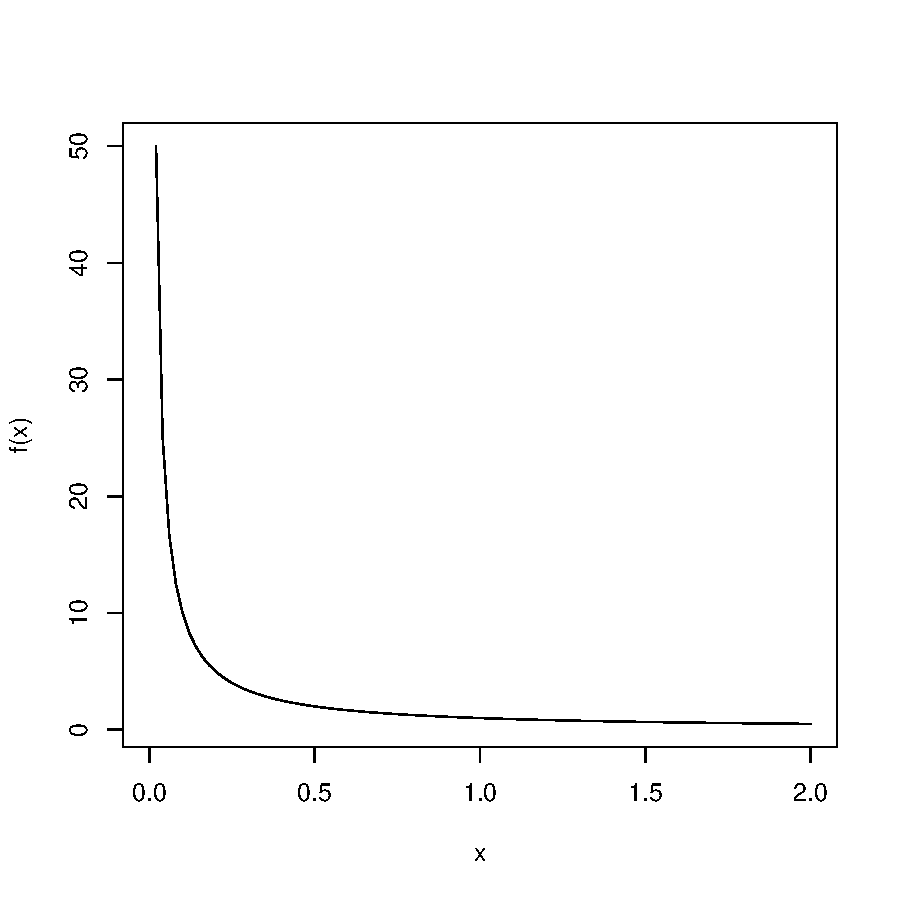
\includegraphics{Rmatematica-062}
\caption{Grafico di $1/x$ nell'intervallo $(0,2)$.}
\label{grafounox}
\end{center}
\end{figure}

Pu\`o essere utile sovrapporre ad un grafico gi\`a tracciato un ulteriore grafico, tracciando ad esempio l'asse $x$, l'asse $y$, o una ulteriore funzione;  la finestra grafica \`e quella preesistente e non deve essere ridefinita ogni volta (si suggerisce di realizzare per primo il grafico con finestra grafica pi\`u ampia). Il parametro da utilizzare in tale caso \`e \texttt{add} (variabile booleana, pu\`o assumere solo valore \texttt{True} o \texttt{False}, indicabili come \texttt{T}  o \texttt{F} o per esteso come \texttt{TRUE}  o \texttt{FALSE}, consigliato), ovviamente nel caso \texttt{F} l'assegnazione del parametro non \`e richiesta). Ad esempio per aggiungere la retta $y=20\,x$ alla funzione precedente si scriver\`a:%%modif i true e false
\begin{Schunk}
\begin{Sinput}
> g<-function(x) 20*x
> curve (g,add=T) 
\end{Sinput}
\end{Schunk}
ottenendo la Figura~\ref{addF}.
\begin{figure}[htbp]
\begin{center}
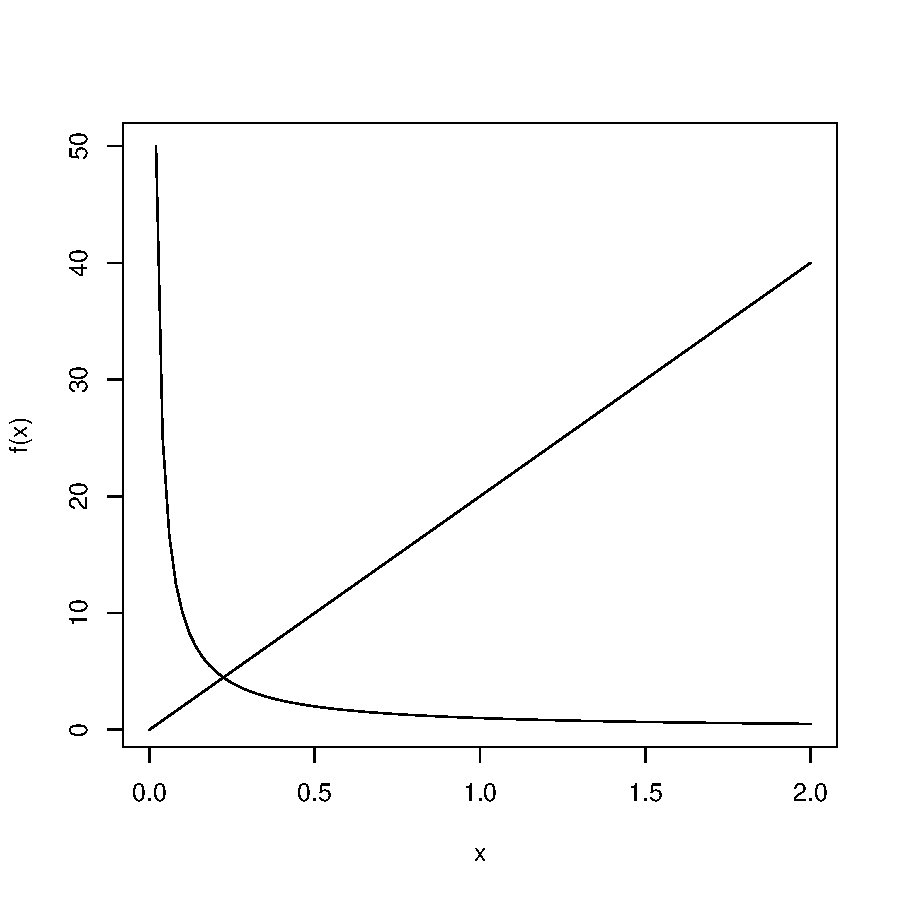
\includegraphics{Rmatematica-065}
\caption{Sovrapposizione di 2 grafici}
\label{addF}
\end{center}
\end{figure}
Vediamo qui di seguito alcune opzioni grafiche:
\begin{itemize}
\item{}Definizione della finestra grafica.\vskip0pt
Possiamo specificare completamente la finestra grafica. 
Per l'asse delle $x$ si ricorre al parametro \texttt{xlim}: $$\texttt{xlim=c}(\varia{estremo inferiore, estremo superiore})$$ 
e in modo simile per l'asse delle $y$ il parametro \`e  \texttt{ylim}:$$\texttt{ylim=c}(\varia{estremo inferiore, estremo superiore})$$
Se ad esempio volessimo tracciare il grafico della funzione precedente  tra -3 e 3 sull'asse $x$ e tra -4 e 4 sull'asse $y$, scriveremo:
\begin{Schunk}
\begin{Sinput}
> curve(1/x,xlim=c( -3,3), ylim=c(-4,4)) 
\end{Sinput}
\end{Schunk}
ed otterremo il grafico della figura~\ref{finestra}.
\begin{figure}[htbp]
\begin{center}
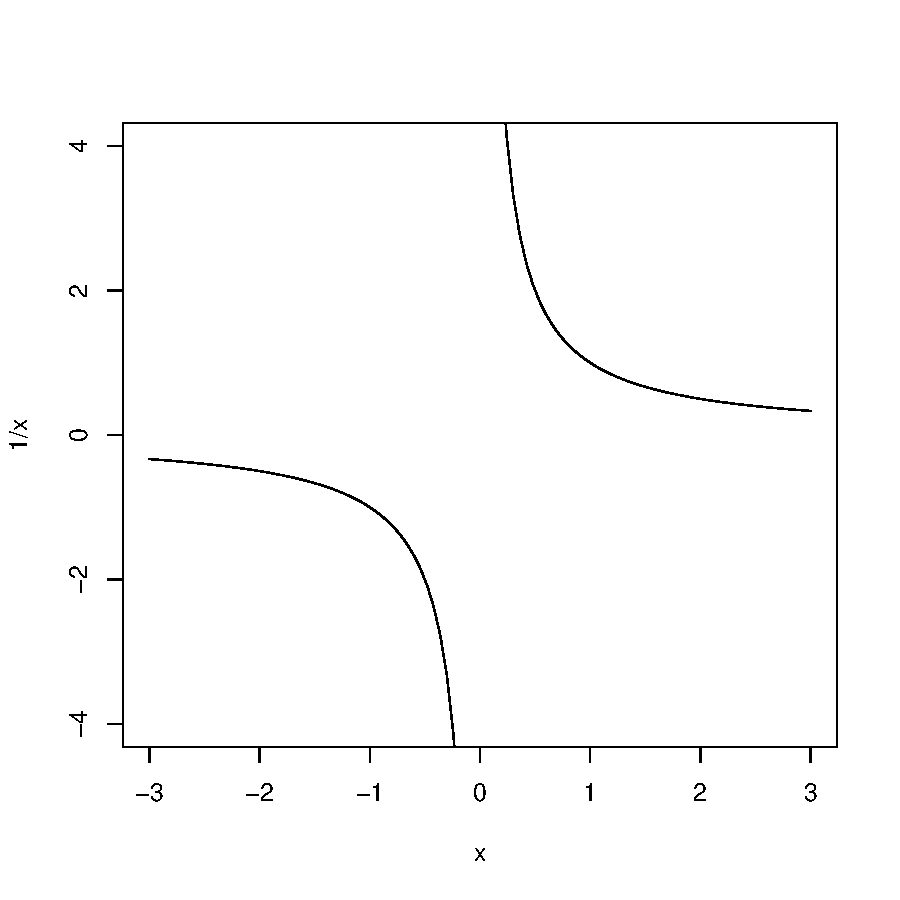
\includegraphics{Rmatematica-067}
%\includegraphics[scale=0.4]{grafici/Rplot34.pdf}
\caption{Scelta della finestra grafica}
\label{finestra}
\end{center}
\end{figure}
Se vogliamo restringere il grafico  tra -2, e 2 della finiestra grafica precedente possiamo scrivere
\begin{Schunk}
\begin{Sinput}
> curve(1/x,from=-2,to=2,xlim=c( -3,3), ylim=c(-4,4)) 
\end{Sinput}
\end{Schunk}
ed otterremo il grafico della figura~\ref{finestra2}.
\begin{figure}[htbp]
\begin{center}
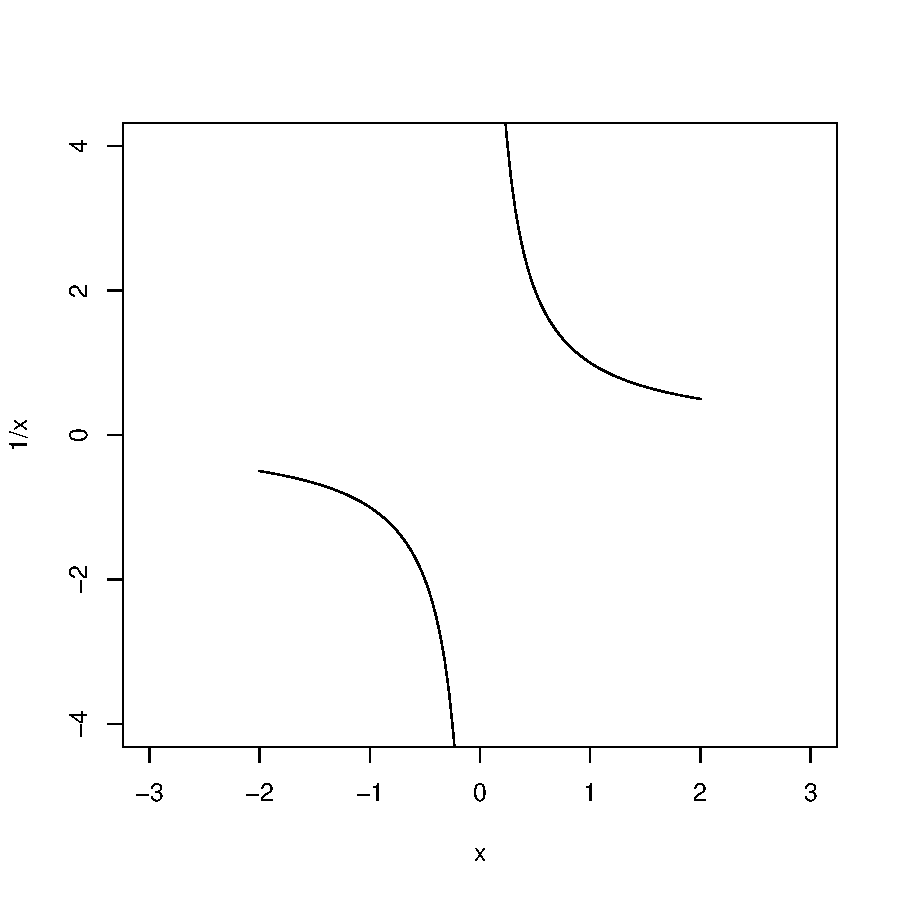
\includegraphics{Rmatematica-069}
%\includegraphics[scale=0.4]{grafici/Rplot34.pdf}
\caption{Scelta della finestra grafica: grafico con dominio ristretto}
\label{finestr2}
\end{center}
\end{figure}
\item{}Selezione del colore della curva.\vskip10pt
Per cambiare il colore predefinito del grafico si deve utilizzare il parametro \texttt{col},  scrivendo  \texttt{col}(\texttt{\virgolette nome colore\virgolette)}.
Il nome del colore deve essere definito in lingua inglese. Per visualizzare l'elenco completo dei colori disponibili si usa il comando: 
\texttt{colors()}.
Tra i principali colori troviamo \par 
\begin{center}
\begin{tabular}{|r| p{2cm} |}
\hline
rosso & red\\
blu & blue\\
bianco & white\\
rosa	&pink\\
verde & green\\
giallo & yellow\\
viola	&purple\\nero	&black\\  \hline
\end{tabular}
\end{center}
\vskip10pt
Sono utilizzabili anche i parametri \texttt{light} e \texttt{dark}, esse devono precedere il nome del colore. Possiamo pensare di colorare la curva precedente di blu scuro e scrivere: 
Otteniamo la  figura~\ref{colori}.
\begin{figure}[phtb]
\begin{center}
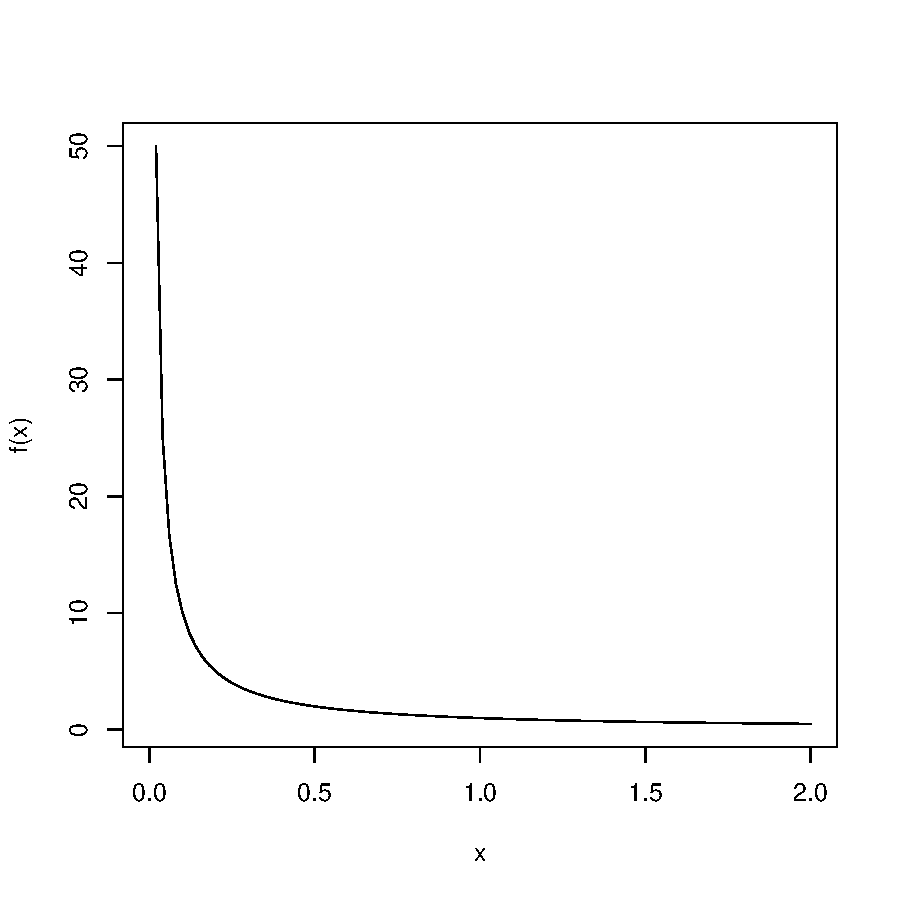
\includegraphics{Rmatematica-071}
\caption{Scelta del colore}
\label{colori}
\end{center}
\end{figure}
Si noti che la dicitura \texttt{dark blue} e \texttt{darkblue} senza spazi producono lo stesso risultato (sono implementati ambo i colori) %%new.
\item{}Selezione dello spessore delle linee

Per cambiare lo spessore delle linee \`e possibile utilizzare il parametro \texttt{lwd}, esso pu\`o avere valori in una scala da 0 fino ad un numero qualunque (anche decimale) di {\it pixel}, se vogliamo  visualizzare la curva precedente con spessore della linea pari a 5 pixel, scriveremo: 

\begin{Schunk}
\begin{Sinput}
> curve(1/x,xlim=c( -3,3),ylim=c(-4,4),col="darkblue", lwd=5)
\end{Sinput}
\end{Schunk}

Otteniamo la figura~\ref{spessore}
\begin{figure}[ htbp]
\begin{center}
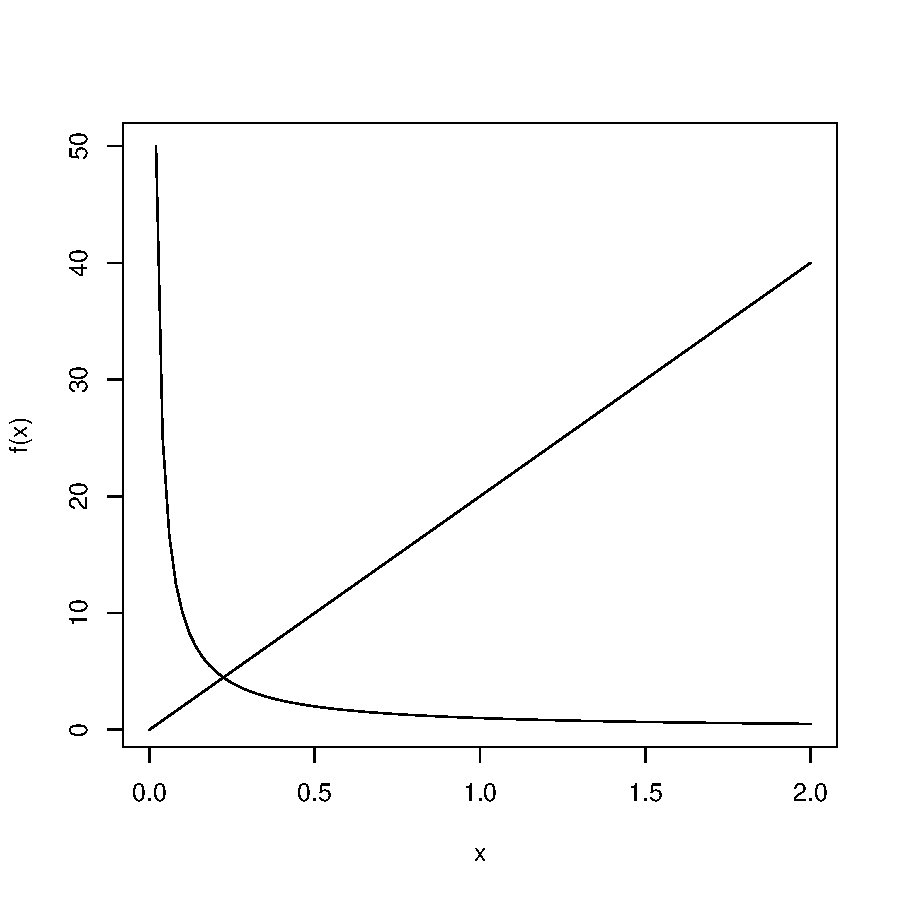
\includegraphics{Rmatematica-074}
\caption{Spessore delle linee}
\label{spessore}
\end{center}
\end{figure}
\item{}Scelta del tipo di linea.\vskip0pt
\`E  possibile scegliere un numero di punti da visualizzare ed \`e anche possibile collegarli o meno. Per scegliere il numero di punti si usa il parametro \texttt{n} associandogli un numero intero.
Per non collegare i punti si usa il parametro \texttt{type}, e si fa assumere valore \texttt{\virgolette p\virgolette}, si scrive quindi: \texttt{type=  \virgolette p\virgolette}.
Ad esempio se vogliamo un numero di punti pari a 100, non collegati, scriveremo:
\begin{Schunk}
\begin{Sinput}
> curve(1/x,xlim=c(-3,3),ylim=c(-4,4), 
+ col="dark blue", lwd=2,n=100,type="p")
\end{Sinput}
\end{Schunk}
il cui risultato \`e riportato in figura~\ref{graficopunti}.
\begin{figure}[ htbp]
\begin{center}
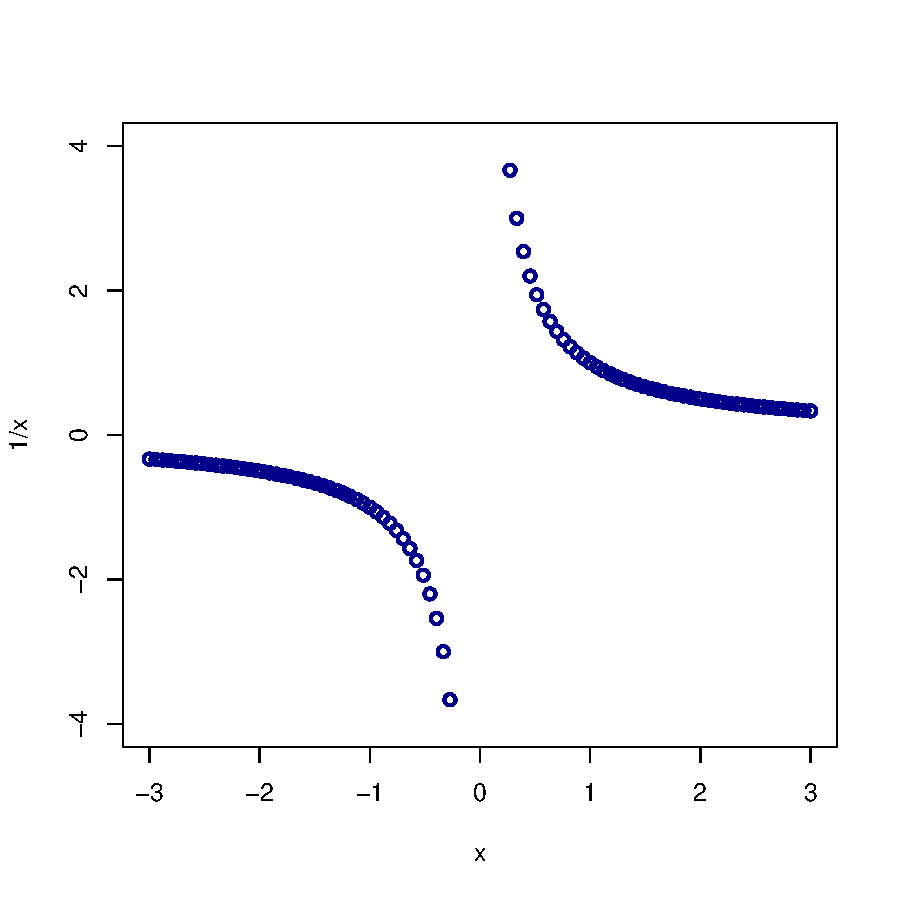
\includegraphics{Rmatematica-078}
%\includegraphics[scale=0.4]{grafici/RplotAPUNTI.pdf}
\caption{Grafico a punti}
\label{graficopunti}
\end{center}
\end{figure}
Altre scelte possibili sono \texttt{type=\virgolette n\virgolette} per il punto non vuoto ma anche \texttt{type=\virgolette l\virgolette} per le linee (scelta di default) e \texttt{type=\virgolette o\virgolette} per punti e linee. 
 

 

\item{} La funzione  \texttt{abline}.

La funzione \texttt{abline}, di sintassi:  
\texttt{abline}(\varia{b,a})
consente di tracciare una retta di pendenza \varia{a} e di intercetta \varia{b}. Se scriviamo \texttt{abline(h}=\varia{valore})
otteniamo una linea orizzontale a quota \varia{valore} mentre con: %%:
\texttt{abline(v=}\varia{valore}) otteniamo una retta verticale ad ascissa  pari al \varia{valore}. Dopo avere tracciato un grafico si possono quindi aggiungere con i  comandi:%%:
\texttt{abline(h=0)}
e \texttt{abline(v=0)}
cio\`e gli assi di riferimento del sistema cartesiano (utili nel caso ad esempio in cui si debbano individuare le intersezioni con gli assi della funzione). Ad esempio se scriviamo:

\begin{Schunk}
\begin{Sinput}
>  curve(1/x,xlim=c( -3,3),
+  ylim=c(-4,4),col="darkblue",lwd=5);
>  abline(h=0);abline(v=0);
\end{Sinput}
\end{Schunk}

Otteniamo la figura~\ref{assisb}.
\begin{figure}[ htbp]
\begin{center}
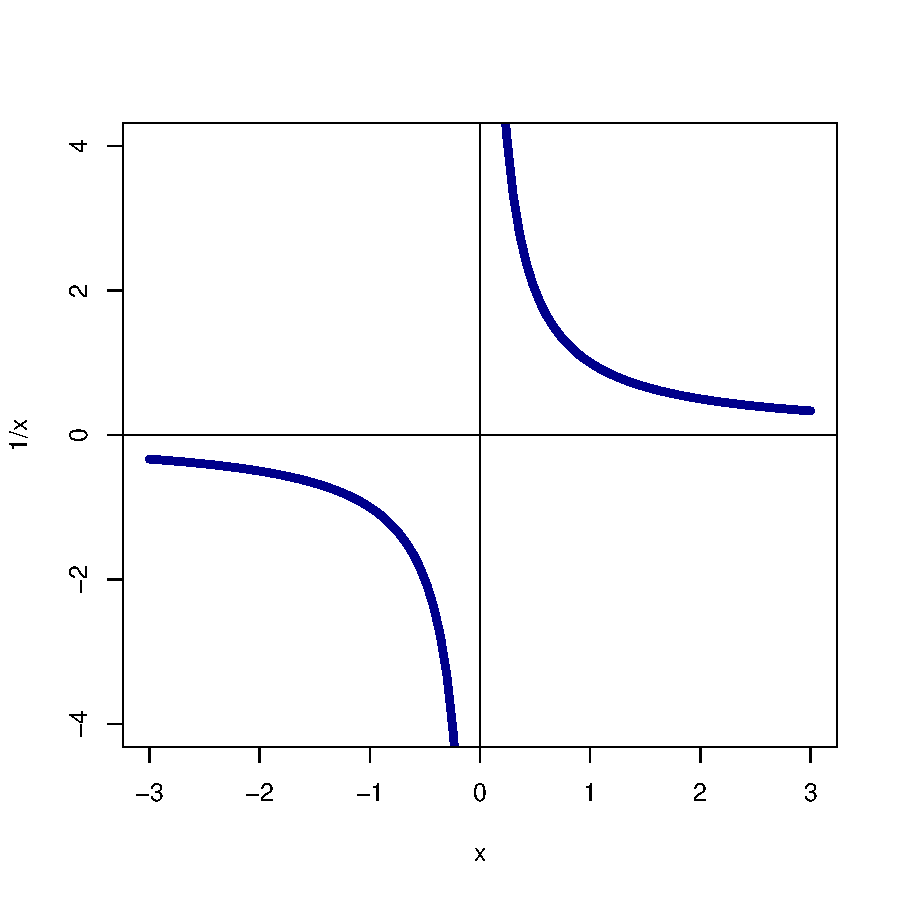
\includegraphics{Rmatematica-082}
\caption{Iperbole con assi}
\label{assisb}
\end{center}
\end{figure} 
Notiamo che cambiando di poco la finestra grafica
\begin{Schunk}
\begin{Sinput}
>  curve(1/x,xlim=c( -3,3.1),
+  ylim=c(-4,4),col="darkblue",lwd=5);
>  abline(h=0);abline(v=0);
\end{Sinput}
\end{Schunk}
Otteniamo la figura~\ref{assisb2}.
\begin{figure}[ htbp]
\begin{center}
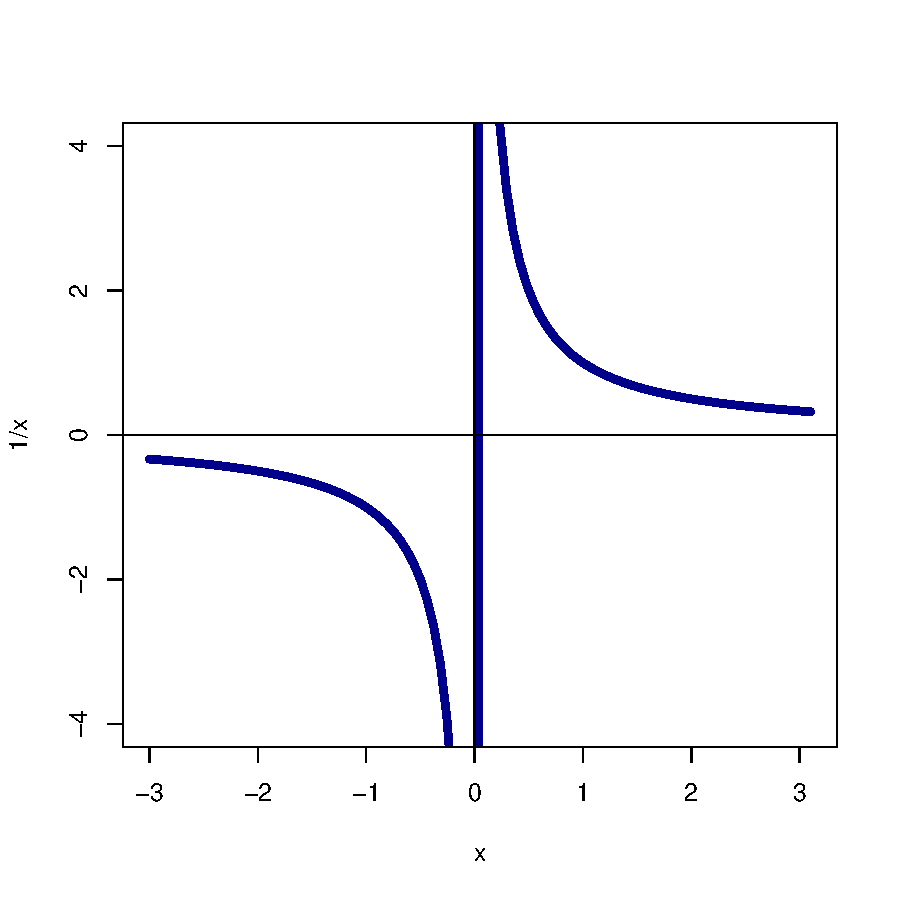
\includegraphics{Rmatematica-086}
 \caption{Problemi grafici}
\label{assisb2}
\end{center}
\end{figure} 

In questa figura una porzione del grafico \`e stata sovraimpressa all'asse verticale.  In effetti uno \`e fittizio determinato dal fatto che la funzione non \`e definita in $x=0$ e che \rpr nel tracciare il grafico cerca di congiungere l'ultimo punto a sinistra dello zero ed il primo a destra. Per eliminare questo problema si pu\`o ricorrere ai comandi che seguono, che generano la figura~\ref{fig:noasint}:.
\begin{Schunk}
\begin{Sinput}
>  curve(1/x, xlim=c( -3,3.1),ylim=c(-4,4),type="n")
>  curve(1/x,xlim=c(-3,0), ylim=c(-4,4), col="darkblue",lwd=5,add=T)
>  curve(1/x,xlim=c(0,3.1),  ylim=c(-4,4),col="darkblue", lwd=5,add=T)
>  abline(h=0,col="red"); abline(v=0,col="red")
\end{Sinput}
\end{Schunk}
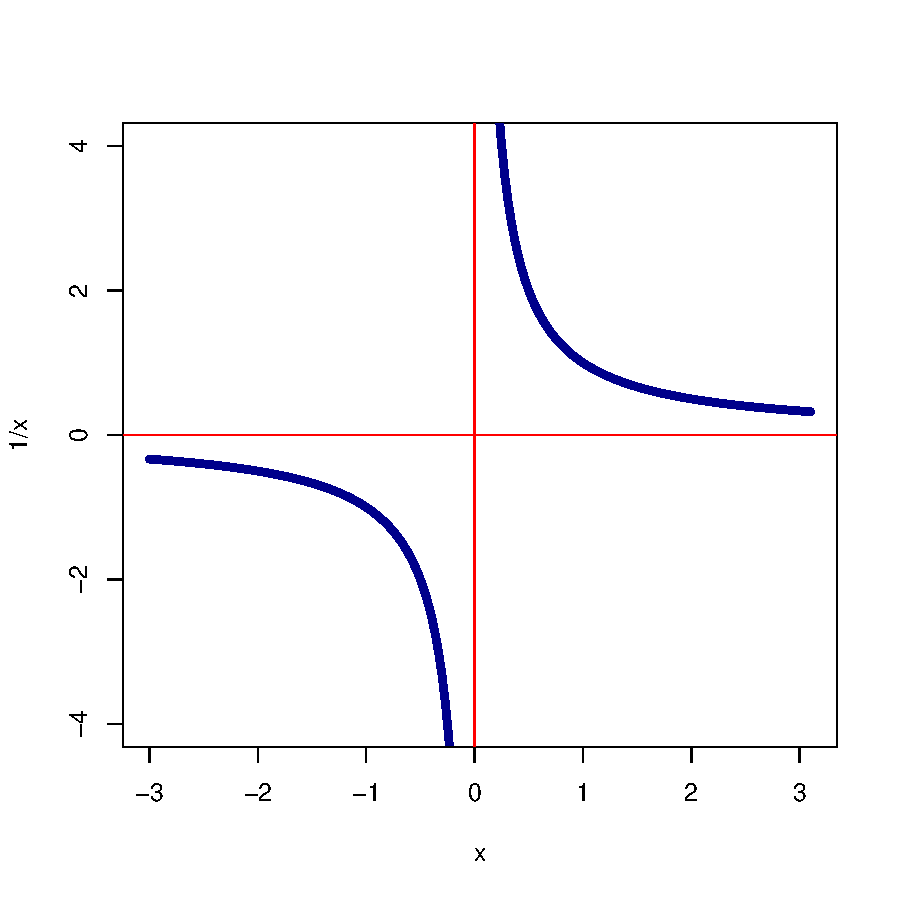
\includegraphics{Rmatematica-088}
\begin{figure}[ htbp]
\begin{center}

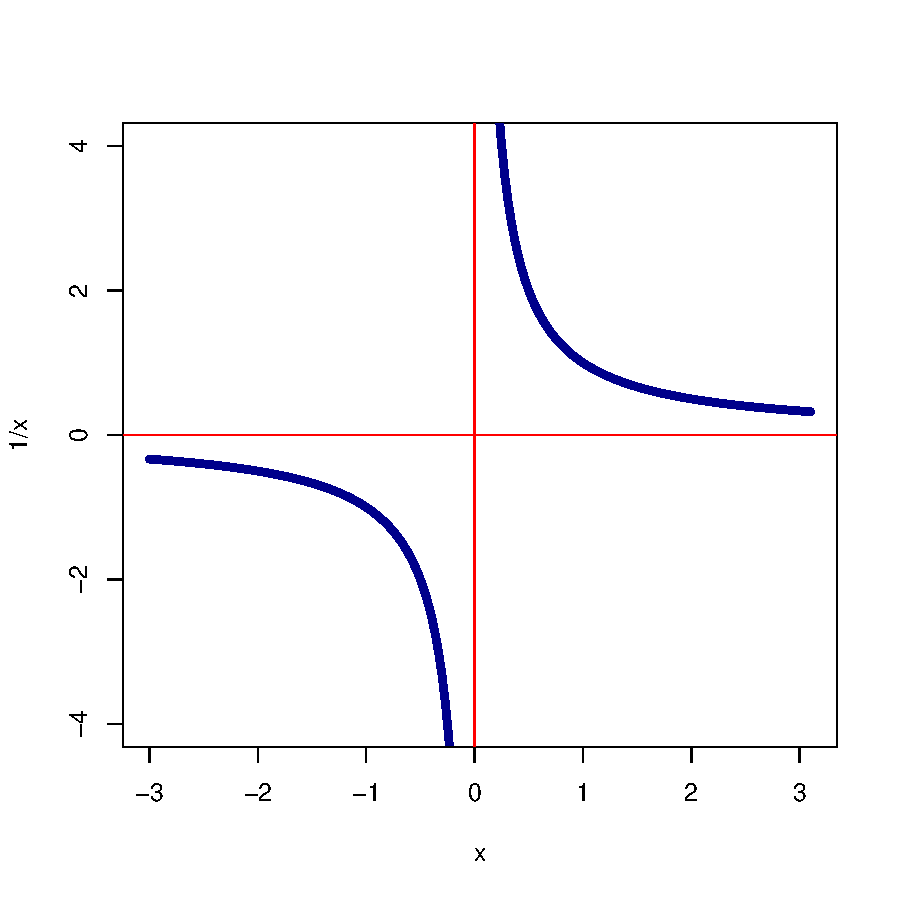
\includegraphics{Rmatematica-089}
%\includegraphics[scale=0.4]{grafici/Rplotsenzaasintoto.pdf}
\caption{Grafico con assi e senza asintoto}
\label{fig:noasint}
\end{center}
\end{figure}
\end{itemize}
\end{itemize}


\section{Composizione di funzioni}
Se abbiamo  le funzioni
\[f\colon D_X   \rightarrow D_Y\]
e
\[g\colon D_{Y'}   \rightarrow D_Z\]
qualora i valori nell'immagine di $f$ siano nel dominio di $g$  (se $\mathrm{Im(f)}  \subseteq D_{Y'}$,cosa garantita se $D_Y=D_{Y'}$ ) possiamo usare l'uscita $y=f(x)$ di $f $ come ingresso della funzione $g$ e possiamo calcolare quindi
 $g(y)=g(f(x))$.
 La funzione cos\'\i~costruita si chiama funzione composta di $f$ e $g$ e viene indicata come
 $g\circ f$. 
 Abbiamo quindi
 \begin{align} g\circ f&\colon D_X\rightarrow D_Z\\
 &x\mapsto y=g(f(x))\end{align}
 
 
\subsection{Esempi}
Si consideri la funzione composta $g\circ f$ delle funzioni $f(x)=x^3+3 \cdot x+1$ e $g(x)=\tan(x)+2$.
Si calcoli $(g\circ f)(4)$. Con R chiamando gf la funzione $g\circ f$
\begin{Schunk}
\begin{Sinput}
> f<-function(x) x^3+3*x+1
> g<-function (x)  tan(x)+2
> gf<-function(x) g(f(x))
> gf(4)
\end{Sinput}
\begin{Soutput}
[1] -30.26858
\end{Soutput}
\end{Schunk}
\section{Funzioni inverse}
Ricordiamo che una funzione $f\colon D_X\rightarrow D_Y$
\`e invertibile se comunque si scelga $y\in D_Y$ la soluzione $x$ in $D_X$ dell'equazione
\[f(x)=y \]
nella variabile $x$ esiste ed \`e unica. 
\\
In tale situazione la funzione inversa esiste \`e denotata con $f^{-1}$ ed  \`e definita come
\begin{align}     f^{-1}&\colon D_Y\rightarrow D_X
\\
&y\mapsto x=f^{-1}(y) \hbox{ $\mid x$ soluzione unica di } f(x)=y\end{align}
\\
Ne segue che ad un arbitrario $y\in D_Y$  possiamo associare in modo unico $x\in D_X$ tale che $f(x)=y$  e quindi
$(f\circ f^{-1})(y)=f(f^{-1}(y))=f(x)=y$  mentre se $x \in D_X$ $(f^{-1}\circ f)(x)= f^{-1}(f(x))=f^{-1}(y)=x$.  Quindi
\begin{align}  f\circ f^{-1}&\colon D_Y\rightarrow D_Y
\\
&x\mapsto f(f^{-1}(y))=y\end{align}
 e
\begin{align} f^{-1} \circ f&\colon D_X\rightarrow D_X
\\
&x\mapsto f^{-1}(f(x))=x\end{align}
sono le funzioni identiche di dominio e codominio rispettivamente.
\begin{itemize}
\item Si calcoli 
\[5^{3/2 \log_{5}(4)}\]
\end{itemize}
\subsection{Grafico delle funzioni inverse}
Il grafico di una funzione invertible 
$f\colon D_X\rightarrow D_Y$ \`e
l'insieme di punti nel piano 
\[\Gamma_f=\{(x,f(x))\mid x \in D_X\}\]
In modo simile il grafico di $f^{-1}$ \`e l'insieme di punti
\[\Gamma_{f^{-1}}=\{(y,f(y))\mid y \in D_Y\}\]
ma poich\'e l'equazione $f(x)=y$ ha una e una sola soluzione $x\in D_X$
\[\{(y,f^{-1}(y))\mid y \in D_Y\}=\{(f(x),f^{-1}(f(x))\mid x \in D_X\}=\{(f(x),x)\mid x \in D_X\}\]

Per ottenere il grafico della funzione inversa a partire dal grafico basta quindi trovare una trasformazione del piano che trasformi l'asse $x$ nell'asse $y$ e viceversa. Una possibile realizzazione di tutto questo \`e ripostato nella figura \ref{fig::simmetria}
\begin{figure}
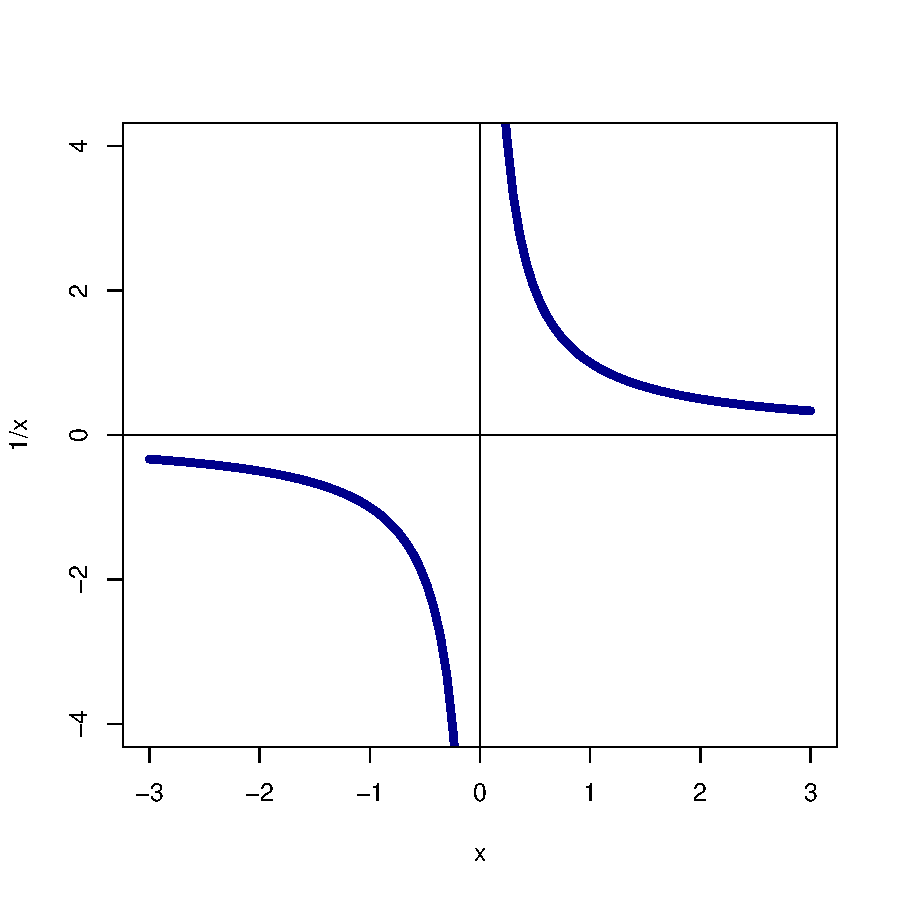
\includegraphics{Rmatematica-091}

\caption{Trasformazione che consente di passare dal grafico di una funzione al grafico della sua funzione inversa}
\label{fig::simmetria}
  \end{figure}
Come si pu\`o realizzare concretamente questa trasformazione?
\\
Partiamo per esempio dal grafico riportato in Figura~\ref{fig::funzionestart}
\begin{figure}
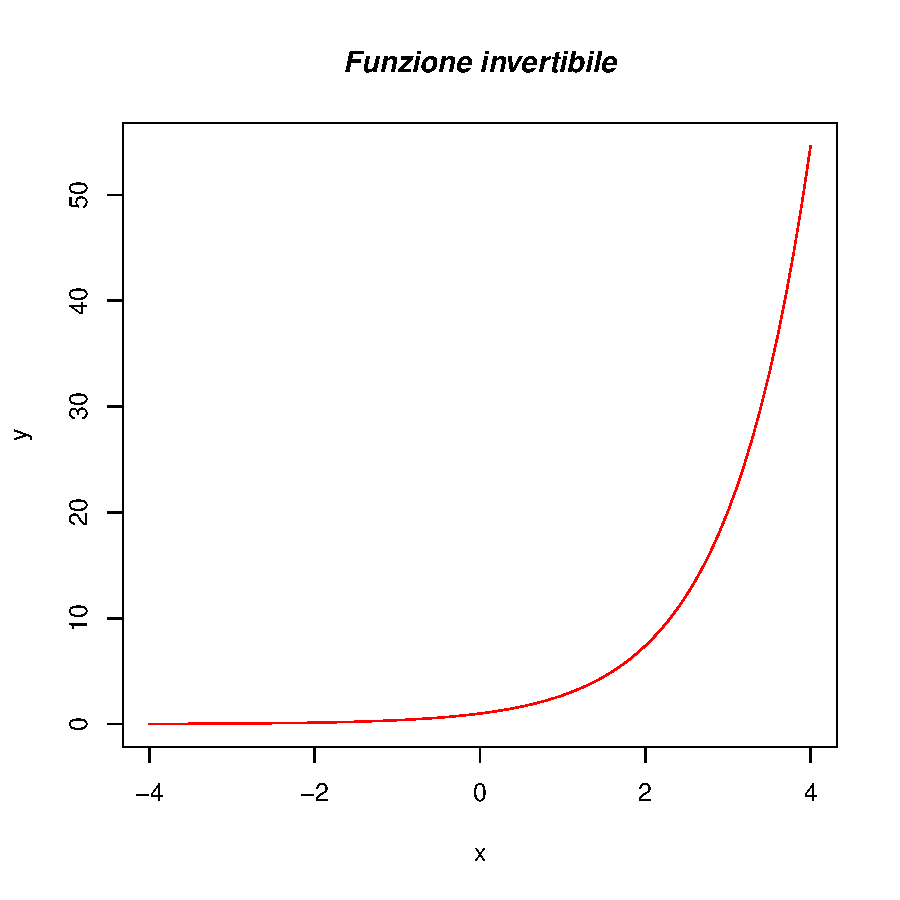
\includegraphics{Rmatematica-092}
\caption{Grafico di una funzione invertibile (esponenziale)}
\label{fig::funzionestart}
\end{figure}
\begin{figure}

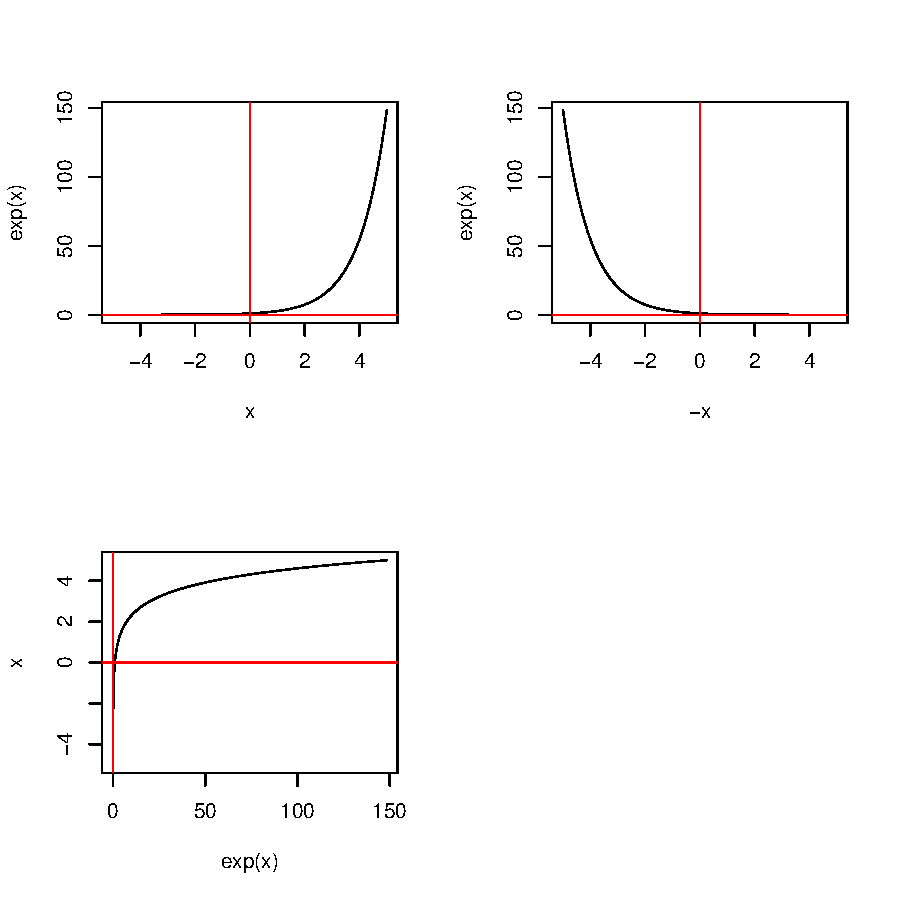
\includegraphics{Rmatematica-093}
\end{figure}
possiamo partire da una sequenza regolare di punti del dominio  di $f$ ed eseguire le trasformazioni  
\begin{itemize}
\item Cambiare $x$ in $-x$
\item Cambiare $(x,f(x))$ in $(f(x),x)$
\end{itemize}
Nell'esempio abbiamo scelto come dominio l'intervallo $[-4,4]$. Abbiamo quindi costruito una seguenza di punti in tale intervallo e poi eseguito i comandi
\begin{Schunk}
\begin{Sinput}
> par(mfrow=c(2,2))
> x=seq(-4,4,0.1)
> y=exp(x)
> plot(x,y,type="l");abline(h=0,col="red");abline(v=0,col="red")
> plot(-x,y,type="l");abline(h=0,col="red");abline(v=0,col="red")
> plot(y,x,type="l");abline(h=0,col="red");abline(v=0,col="red")
> par(mfrow=c(1,1))
\end{Sinput}
\end{Schunk}
Qui il comando \texttt{plot(x,y)} rappresenta i punti di coordinate $(x,y)$ nel piano.
\section{Funzioni inverse delle funzioni circolari}

Come visto a lezione le funzioni seno, coseno e tangente non sono invertibili; se per\`o consideriamo opportune restrizioni di tali funzioni, possiamo costruire le funzioni arcoseno, arcocoseno e arcotangente. Pi\`u precisamente
la restrizione della funzione \texttt{sin}
$$\sin\colon [-\frac{\pi}{2},\frac{\pi}{2}]\rightarrow [-1,1]$$
\`e invertibile e la sua funzione inversa \`e  la funzione arcoseno, che indicheremo con \texttt{asin}
$$\texttt{asin}\colon  [-1,1]\rightarrow [-\frac{\pi}{2},\frac{\pi}{2}]$$
\begin{figure}

\begin{Schunk}
\begin{Sinput}
> par(mfrow=c(1,2))
> x=seq(-pi/2,pi/2,0.01)
> plot(x,sin(x))
> plot(sin(x),x)
\end{Sinput}
\end{Schunk}
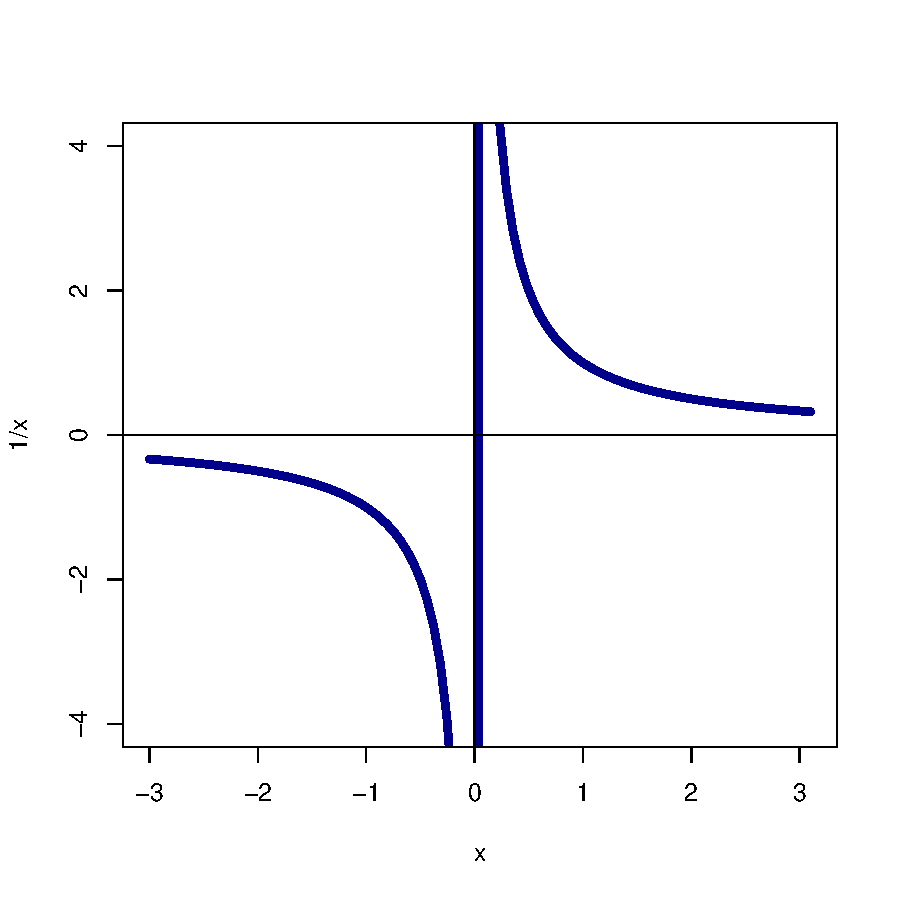
\includegraphics{Rmatematica-095}
\end{figure}
In modo simile la funzione
$$\cos\colon [0,\pi]-\rightarrow [-1,1]$$
 \`e invertibile e la sua funzione inversa \`e  la funzione arcocoseno, che indicheremo con \texttt{acos}
$$\texttt{acos}\colon  [-1,1]\rightarrow [0,\pi]$$
\begin{Schunk}
\begin{Sinput}
> par(mfrow=c(1,2))
> x=seq(0,pi,0.01)
> plot(x,cos(x))
> plot(cos(x),x)
\end{Sinput}
\end{Schunk}
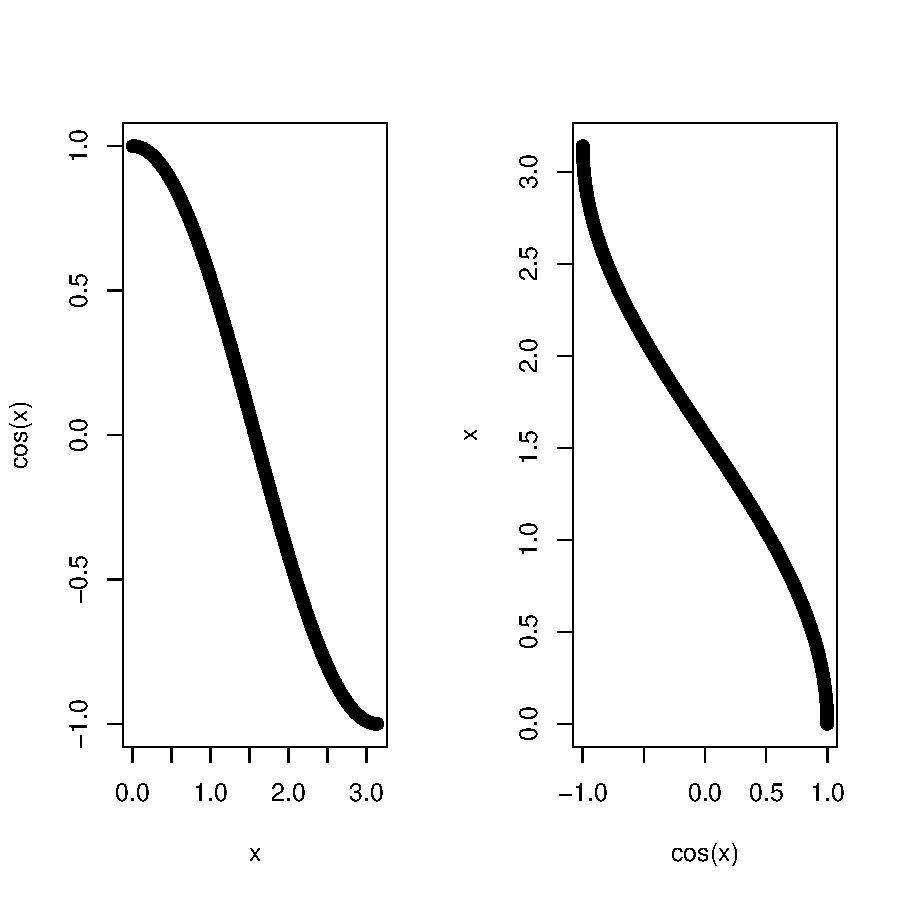
\includegraphics{Rmatematica-096}
e lo \`e pure la funzione
$$\tan\colon (-\frac{\pi}2 ,\frac{\pi}2)\rightarrow \mathbb{R}.$$
La sua funzione inversa \`e  la funzione arcotangente che indicheremo con \texttt{atan}
$$\texttt{atan}\colon  \mathbb R \rightarrow (-\frac{\pi}{2},\frac{\pi}{2})$$
\begin{Schunk}
\begin{Sinput}
> par(mfrow=c(1,2))
> x=seq(-pi/2,pi/2,0.01)
> plot(x,tan(x),ylim=c(-10,10),type="l")
> plot(tan(x),x,type="l",xlim=c(-10,10));abline(h=0);abline(v=0)
\end{Sinput}
\end{Schunk}
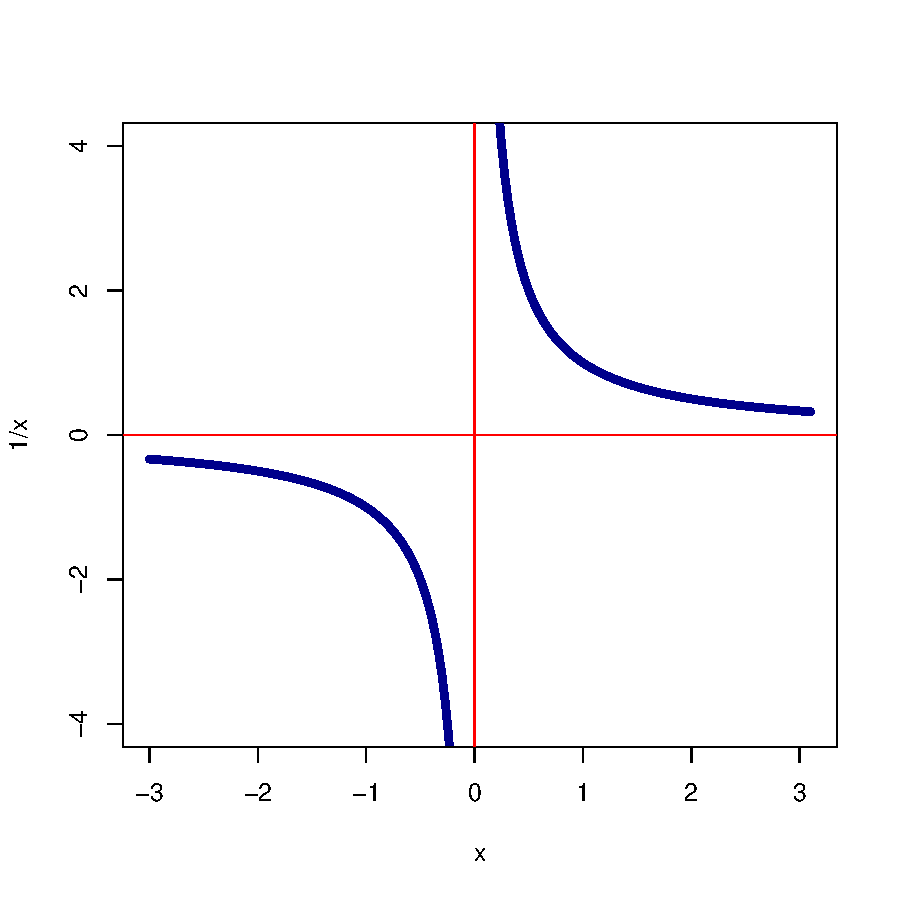
\includegraphics{Rmatematica-097}

\section{Derivate}
Richiamiamo il significato geometrico della derivata: se una funzione $f$ \`e derivabile in un punto $x_0$ allora il grafico si linearizza con un numero sufficiente di ingrandimenti attorno al punto $(x_0,f(x_0))$. 
Come illustrazione di questo processo consideriamo l'iperbole
\begin{Schunk}
\begin{Sinput}
> f<-function(x) 4*x/(2+x)  
\end{Sinput}
\end{Schunk}
e disegniamo il suo grafico nella regione definita dalle condizioni $-d<x<d$ e $-d<y<d$, dove $d$ \`e inizialmente pari a 8.
\begin{Schunk}
\begin{Sinput}
> d=8;curve(f,xlim=c(-d,d),ylim=c(-d,d), main="iperbole"); abline(h=0);abline(v=0)
\end{Sinput}
\end{Schunk}
\begin{figure}
\begin{Schunk}
\begin{Sinput}
> d=8;curve(f,xlim=c(-d,d),ylim=c(-d,d),
> main="iperbole"); abline(h=0);abline(v=0)
\end{Sinput}
\end{Schunk}
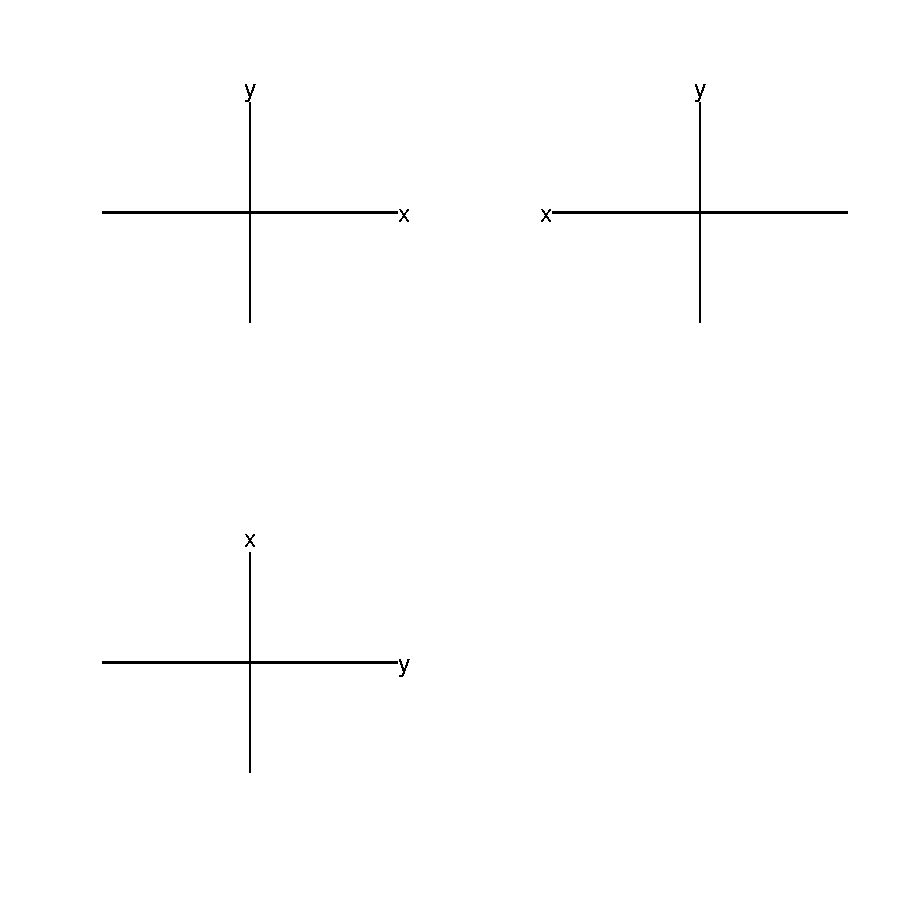
\includegraphics{Rmatematica-100}
\end{figure}

Consideriamo ora l'ingrandimento di tale grafico con fattore di zoom \texttt{xf}=2 attorno al punto $(0,0)$: in altre parole dimezziamo il valore di $d$:
\begin{Schunk}
\begin{Sinput}
> d=d/2;curve(f,xlim=c(-d,d),ylim=c(-d,d),
> main="zoom 2"); abline(h=0);abline(v=0)
\end{Sinput}
\end{Schunk}
Iterando tale comando un certo numero di volte si assiste alla linearizzazione progressiva del grafico come in figura~\ref{fig:lin3}. 
\begin{center}
\begin{figure}
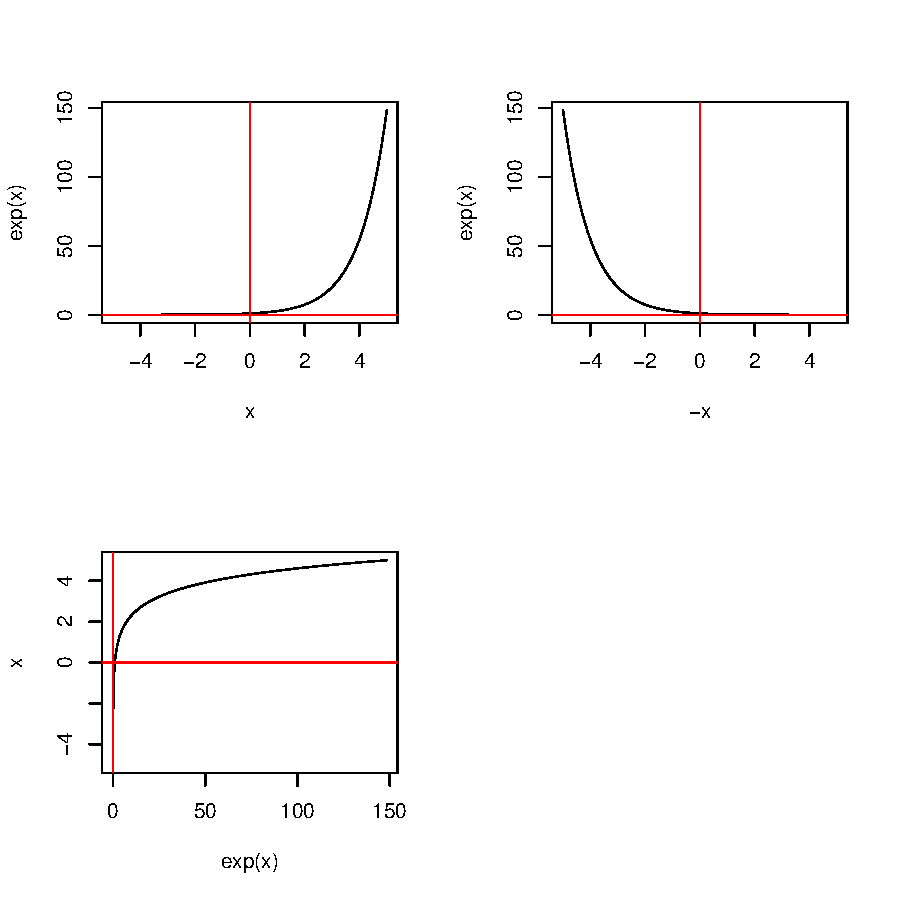
\includegraphics{Rmatematica-102}
\caption{Linearizzazione di un grafico ottenuta attraverso una serie di ingrandimenti}
\label{fig:lin3}
\end{figure}
\end{center}
 
Consideriamo ora una funzione differente che combina un'espressione di quarto grado e una funzione circolare rapidamente oscillante
\begin{Schunk}
\begin{Sinput}
> f<-function(x) x^4/500 + sin(100*x)/100;
\end{Sinput}
\end{Schunk}
Il grafico per $-8<x<8$ come in precedenza  suggerisce che la  retta tangente  in $x=0$ sia orizzontale.   
Effettuando un certo numero di zoom con fattore di zoom 2 questa prima impressione sembra confermata, anche se possiamo iniziare a notare delle piccole oscillazioni nell'ultima figura del pannello~\ref{fig:linear2}.
\begin{figure}
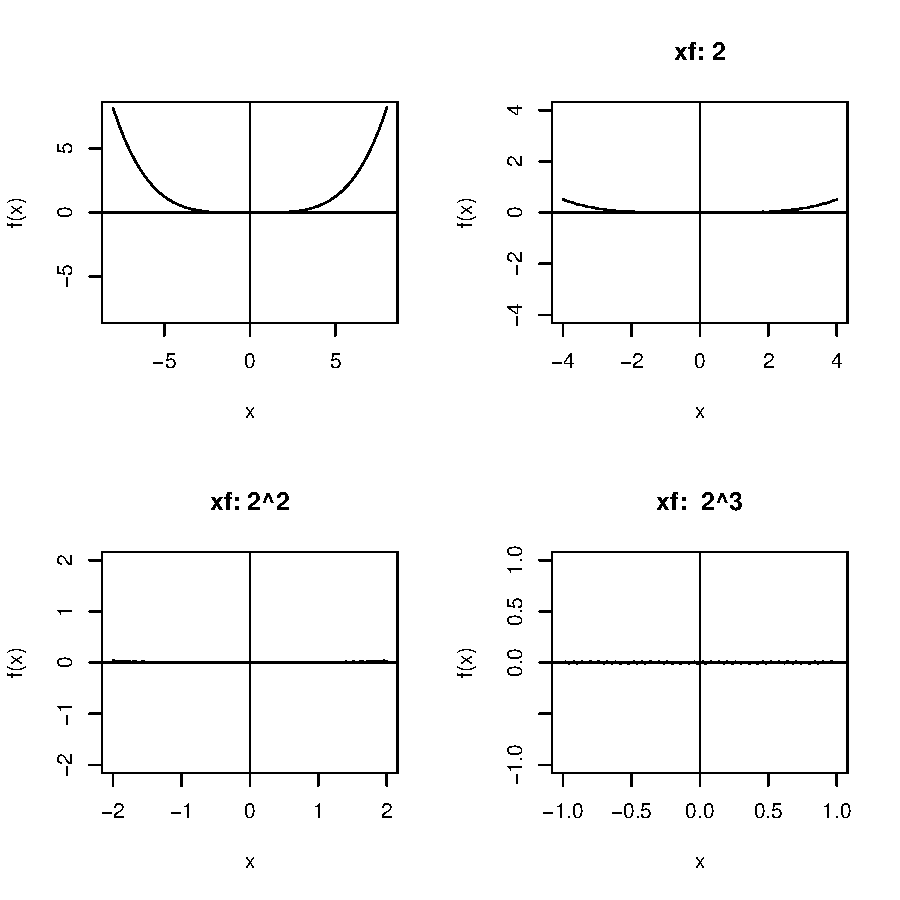
\includegraphics{Rmatematica-104}
\caption{Linearizzazione progressiva di un grafico: prima fase}
\label{fig:linear2}
\end{figure}

Se procediamo con gli ingrandimenti  questa sensazione viene confermata.
Non ci saranno ulteriori sorprese da un certo punto in poi. 
Per quanto si prosegua la retta trovata in ultimo verr\`a confermata~\ref{fig:linearizzazione4}

\begin{figure}[h]
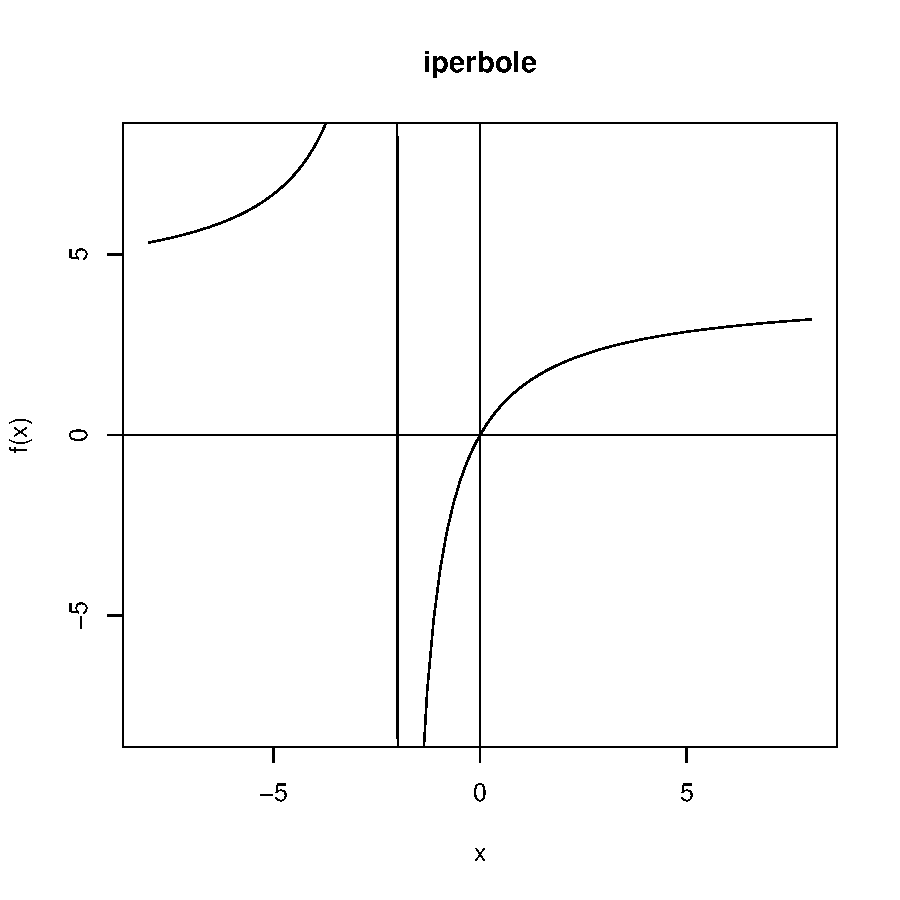
\includegraphics{Rmatematica-105}
\caption{Linearizzazione progressiva di un grafico: seconda fase}
\label{fig:linearizzazione4}
\end{figure}
 \subsection{Regola dei tre punti}
Possiamo stimare la derivata di una funzione $f$ in $x$ con la regola dei tre punti nel punto $x$ con incremento $h$
$$
\texttt{trepunti}(f,x,h)=\frac{f(x+h)-f(x-h)}{2h}
$$
Ora \`e sufficiente definire la funzione di cui vogliamo stimare la derivata, per poi richiamare la funzione \texttt{trepunti} fornendo il valore di $x$ ed il valore dell'incremento $h$.

Approssimiamo ad esempio la derivata di $x\rightarrow {\rm sin}(x)$
Definiamo la funzione e la regola della differenza centrale
\begin{Schunk}
\begin{Sinput}
> f<-function(x) sin(x)
> trepunti<-function(f,x,h) (f(x+h)-f(x-h))/(2*h)
\end{Sinput}
\end{Schunk}
Per esempio assegnando  
\begin{Schunk}
\begin{Sinput}
> h=0.001
> x=1
\end{Sinput}
\end{Schunk}
Si ha 
\begin{Schunk}
\begin{Sinput}
> trepunti(f,x,h)
\end{Sinput}
\begin{Soutput}
[1] 0.5403022
\end{Soutput}
\end{Schunk}
Otteniamo cos\`\i\; la stima della derivata nel punto 1 con incremento 0.001.
Possiamo anche rappresentare graficamente la funzione derivata (insieme alla funzione di \texttt{sin}) scrivendo:
\begin{Schunk}
\begin{Sinput}
> curve(trepunti(f,x,0.001),0,2*pi,col="blue")
> curve(f,add=T,col="red")
\end{Sinput}
\end{Schunk}
e ottenendo il grafico~\ref{sincos} da cui si evince che  $D\rm{sin}(x)={\rm cos}(x)$. In modo simile si pu\`o mostrare che 
$D{\rm cos}(x)=-{\rm sin}(x)$.
\begin{figure}[ htbp]
\begin{center}
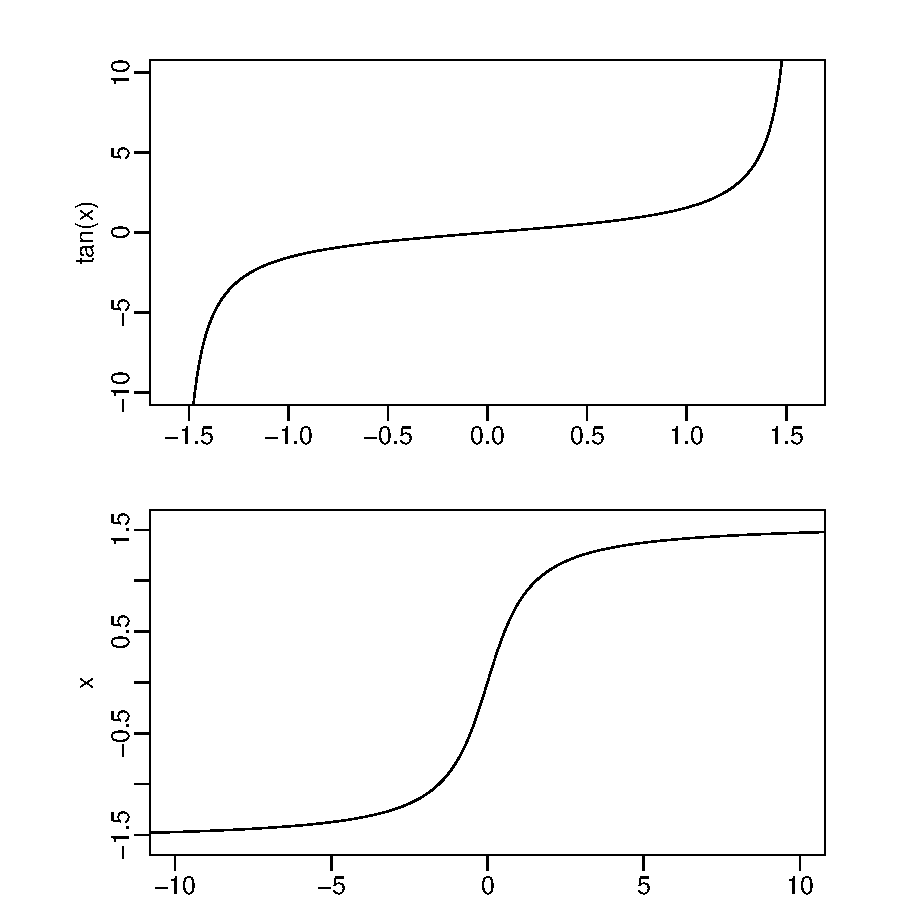
\includegraphics{Rmatematica-110}
\caption{Grafico delle funzioni $sin(x)$ e della sua derivata calcolata numericamente}
\label{sincos}
\end{center}
\end{figure}
Analizziamo ancora la derivata delle funzioni esponenziali. Consideriamo inizialmente
la funzione
$$f(x)=2^x$$ 
In questo caso
\begin{Schunk}
\begin{Sinput}
> f<-function(x) 2^x
> curve(trepunti(f,x,0.001),-2,2,
+ col="blue")
> curve(f,add=T,col="red")
> curve(trepunti(f,x,0.001)/f(x),add=T,
+ col="dark green")
\end{Sinput}
\end{Schunk}
sembra che  la funzione (in rosso) e la sua derivata (in blu, approssimata con la regola dei 3 punti)   siano proporzionali.
\begin{figure}[ htbp]
\begin{center}
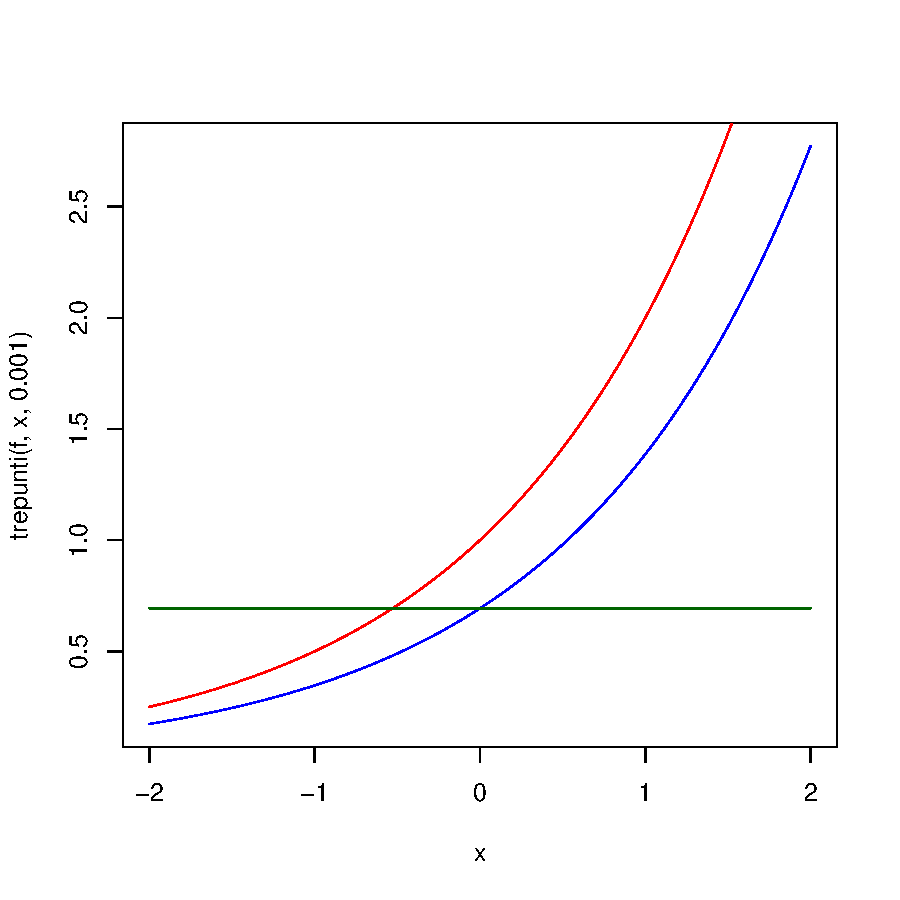
\includegraphics{Rmatematica-112}
\caption{Grafico di $2^x$ e derivata}
\label{fig:der2x}
\end{center}
\end{figure}
Per verificarlo abbiamo tracciato anche il grafico di $f'(x)/f(x)$ che \`e una retta orizzontale a quota
\begin{Schunk}
\begin{Sinput}
>  trepunti(f,0,0.001)/f(0)
\end{Sinput}
\begin{Soutput}
[1] 0.6931472
\end{Soutput}
\end{Schunk}
In modo simile possiamo considerare con la funzione $3^x$:
\begin{Schunk}
\begin{Sinput}
> f<-function(x) 3^x
> curve(trepunti(f,x,0.001),-2,2,col="blue")
> curve(f,add=T,col="red")
> curve(trepunti(f,x,0.001)/f(x),add=T,col="dark green")
\end{Sinput}
\end{Schunk}
e anche qui  le funzioni sembrano proporzionali. In questo caso per\`o il rapporto derivata diviso funzione \`e  maggiore di 1 e quindi la derivata \`e maggiore della funzione
\begin{figure}[ htbp]
\begin{center}
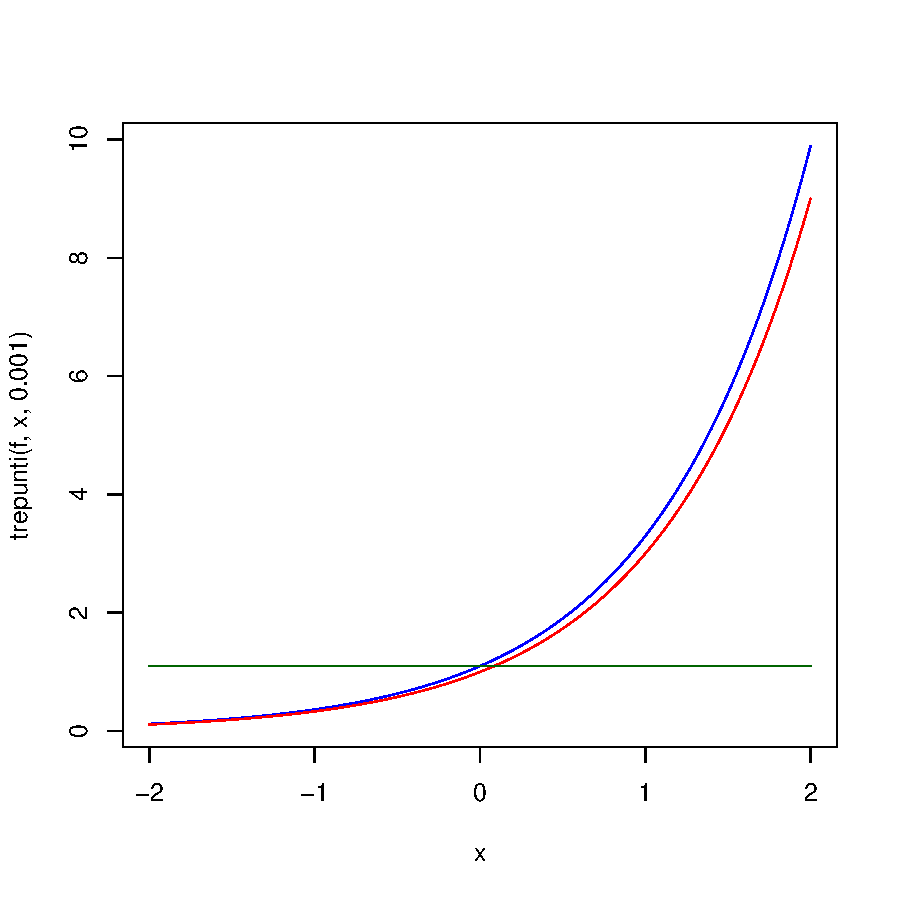
\includegraphics{Rmatematica-115}
\caption{Grafico di $3^x$ e derivata}
\label{fig:der3x}
\end{center}
\end{figure}

Per verificarlo abbiamo tracciato anche il grafico di $f'(x)/f(x)$ che \`e una retta orizzontale a quota
\begin{Schunk}
\begin{Sinput}
> trepunti(f,0,0.001)/f(0)
\end{Sinput}
\begin{Soutput}
[1] 1.098613
\end{Soutput}
\end{Schunk}

Ci si pu\`o chiedere se esista un valore intermedio tra 2 e 3 per cui derivata e funzione coincidano esattamente. La risposta \`e precisamente il numero di Nepero \texttt{exp(1)}. Infatti abbiamo
\begin{Schunk}
\begin{Sinput}
>  f<-function(x) exp(x)
>  curve(trepunti(f,x,0.001),-2,2, col="blue")
>  curve(f,add=T,col="red")
>  curve(trepunti(f,x,0.001)/f(x),add=T, col="dark green")
>  trepunti(f,0,0.001)/f(0)
\end{Sinput}
\end{Schunk}

\begin{figure}
\begin{center}
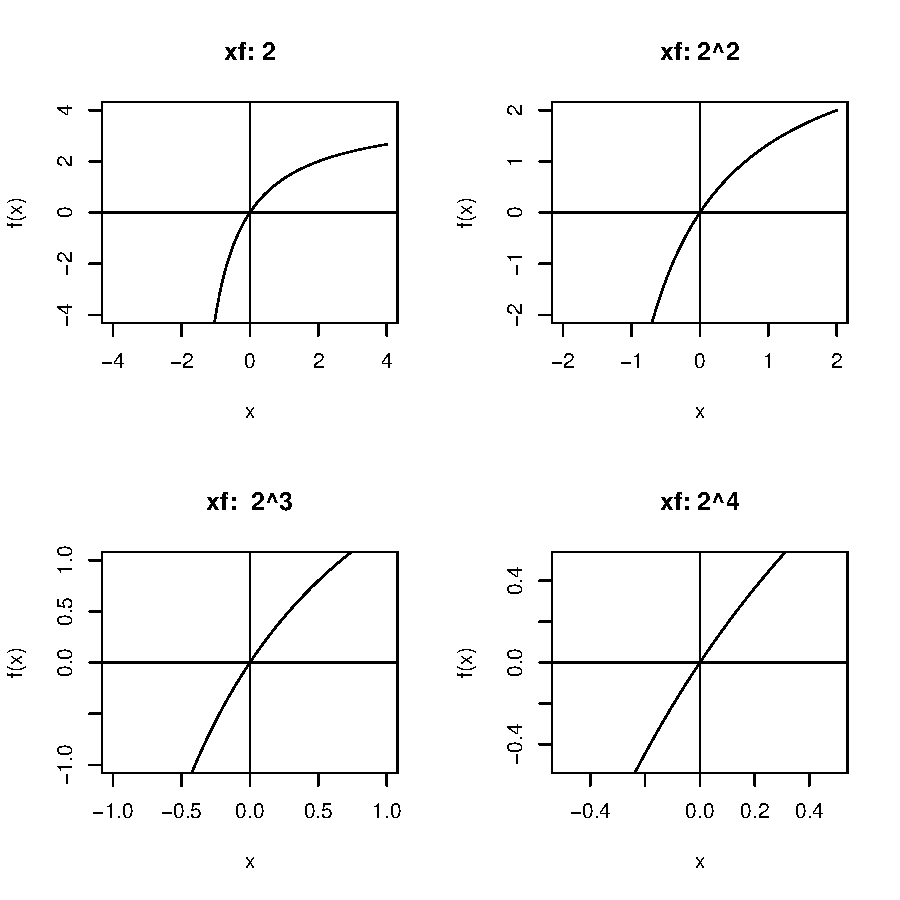
\includegraphics{Rmatematica-118}
\end{center}
\end{figure}

Anche qui
\begin{Schunk}
\begin{Sinput}
> trepunti(f,0,0.001)/f(0)
\end{Sinput}
\begin{Soutput}
[1] 1
\end{Soutput}
\end{Schunk}
mostra il valore del rapporto.

\begin{shaded}
\begin{enumerate}
 \item{ }Ripeti le considerazioni precedenti usando il quoziente di Newton a destra.
\item{} Calcola il valore della approssimazione della derivata con la regola dei tre punti per la funzione $x^2*sin(x)$ in $x=\pi$ con $h=\pi/6$.
\end{enumerate}
\end{shaded}  
\subsection{Derivate ``formali''}
Per calcolare la derivata di una qualunque espressione possiamo scrivere:
\begin{equation*}\texttt{D(expression}(\varia{funzione),variabile})
\end{equation*}
Ad esempio

\begin{Schunk}
\begin{Sinput}
> D(expression(x^4),"x")
\end{Sinput}
\begin{Soutput}
4 * x^3
\end{Soutput}
\end{Schunk}
Un utile comando per valutare una derivata in un punto o per  ricavare una funzione da una derivata \`e il comando \texttt{eval}, ovvero {\it evaluate}. Scriveremo \texttt{eval}(\varia{nome derivata}).

\begin{Schunk}
\begin{Sinput}
> x<-4
> eval(D(expression(x^4),"x"))
\end{Sinput}
\begin{Soutput}
[1] 256
\end{Soutput}
\end{Schunk}

\begin{Schunk}
\begin{Sinput}
> g<-function(x) eval(D(expression(sin(x)),"x"))
> curve(g,0,2*pi)
\end{Sinput}
\end{Schunk}
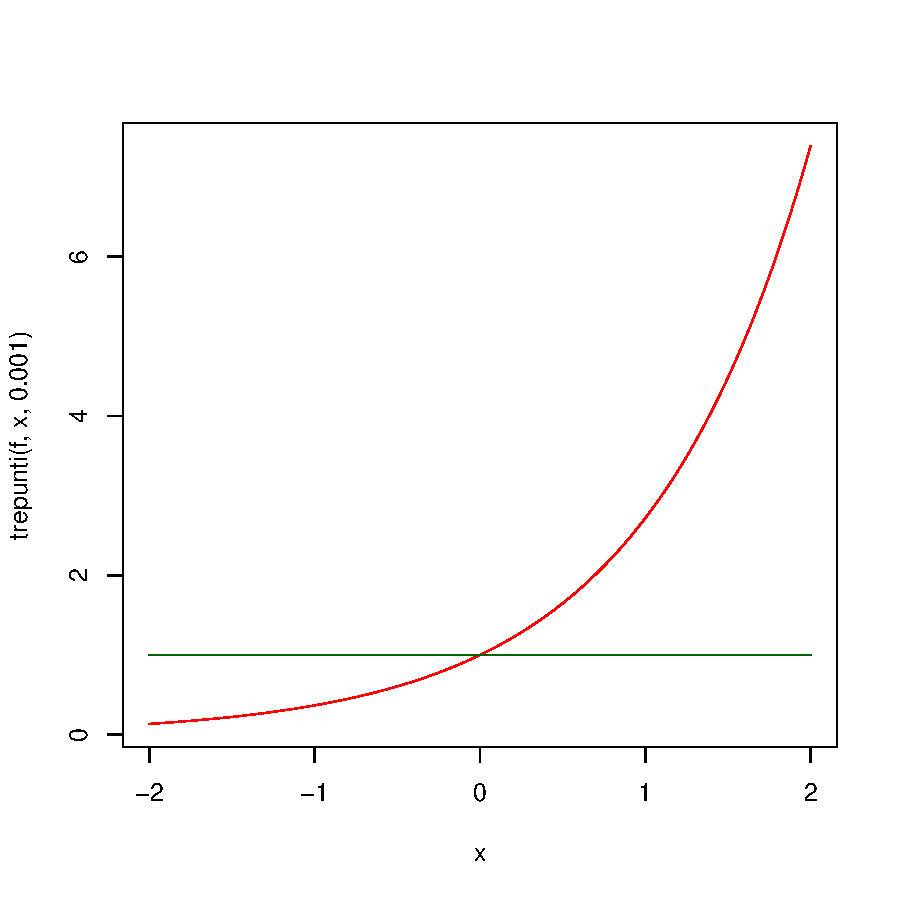
\includegraphics{Rmatematica-122}
\begin{shaded}
\begin{enumerate}
 \item{} Calcola la derivata prima e seconda della funzione $x^2*sin(x)$ in $x=\pi$.
 \item{} Determina l'equazione della retta tangente al grafico della funzione precedente e traccia grafico e retta in una finestra grafica opportuna.
\end{enumerate}
\end{shaded} 
 \subsection{Metodo delle tangenti di Newton}
 Consideriamo ora una funzione generica $f$ il cui grafico presenti delle intersezioni con l'asse delle x
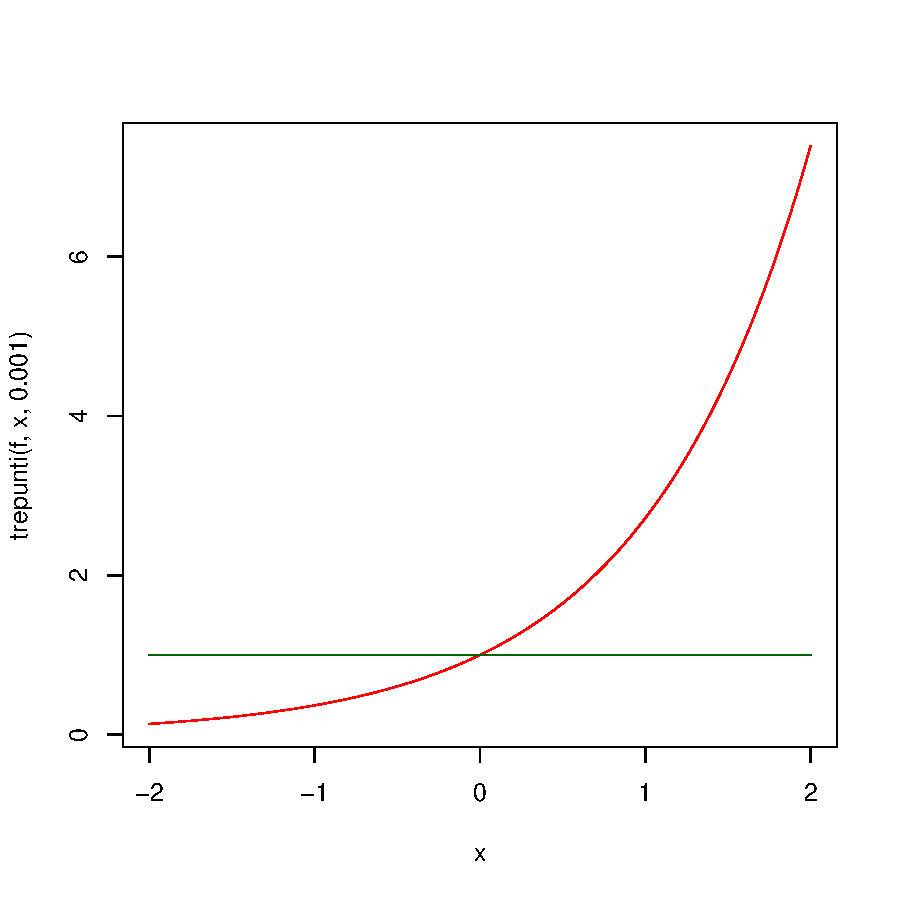
\includegraphics{Rmatematica-123}
Nel metodo delle tangenti di Newton si parte da un'approssimazione iniziale $x_0$, che nel grafico illustrato si situa alla destra di $x_*$.
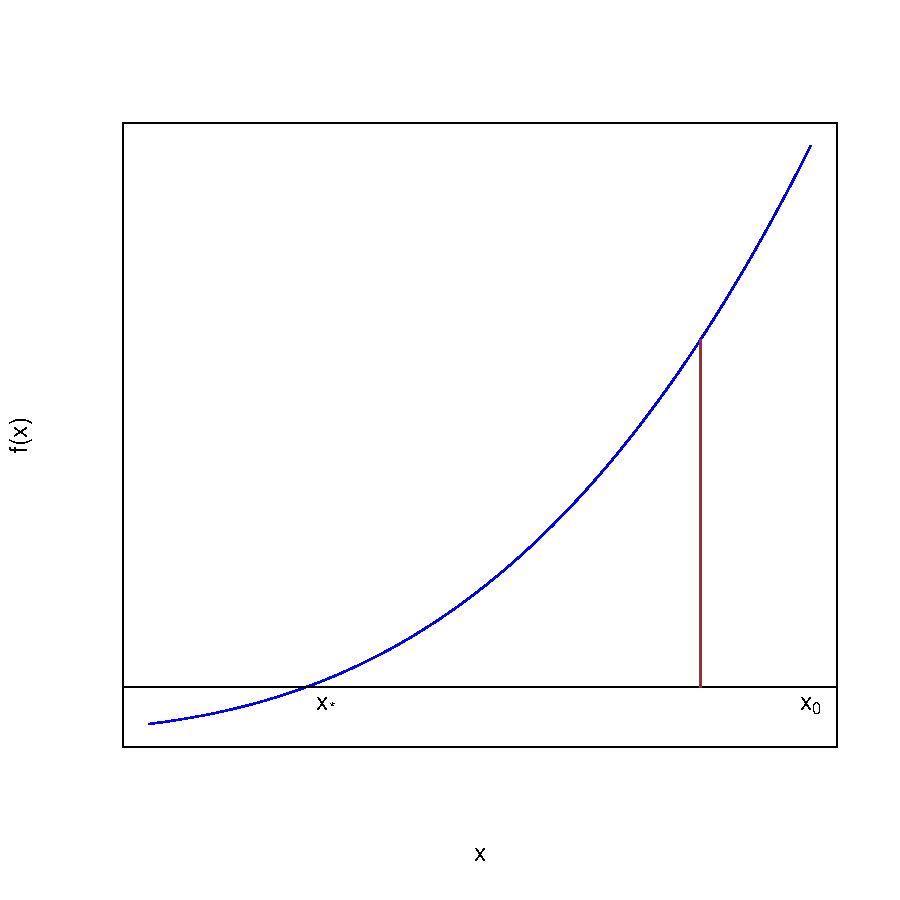
\includegraphics{Rmatematica-124}
Utilizziamo ora il metodo delle tangenti di Newton per determinare gli zeri di una funzione $f$. Prima di iniziare vediamo come possiamo procedere a livello grafico. 
Consideriamo una semplice funzione  $$ f(x)= x^5-3x+1$$
Iniziamo a selezionare una finestra grafica abbastanza ampia. Restringendola man mano vediamo meglio cosa succede.
\begin{Schunk}
\begin{Sinput}
> f<-function(x) x^5-3*x+1
> curve(f,-10,10) 
> abline(h=0)
> curve(f,-2,2)
> abline(h=0)
\end{Sinput}
\end{Schunk}

\begin{figure}[htbp]
\begin{center}
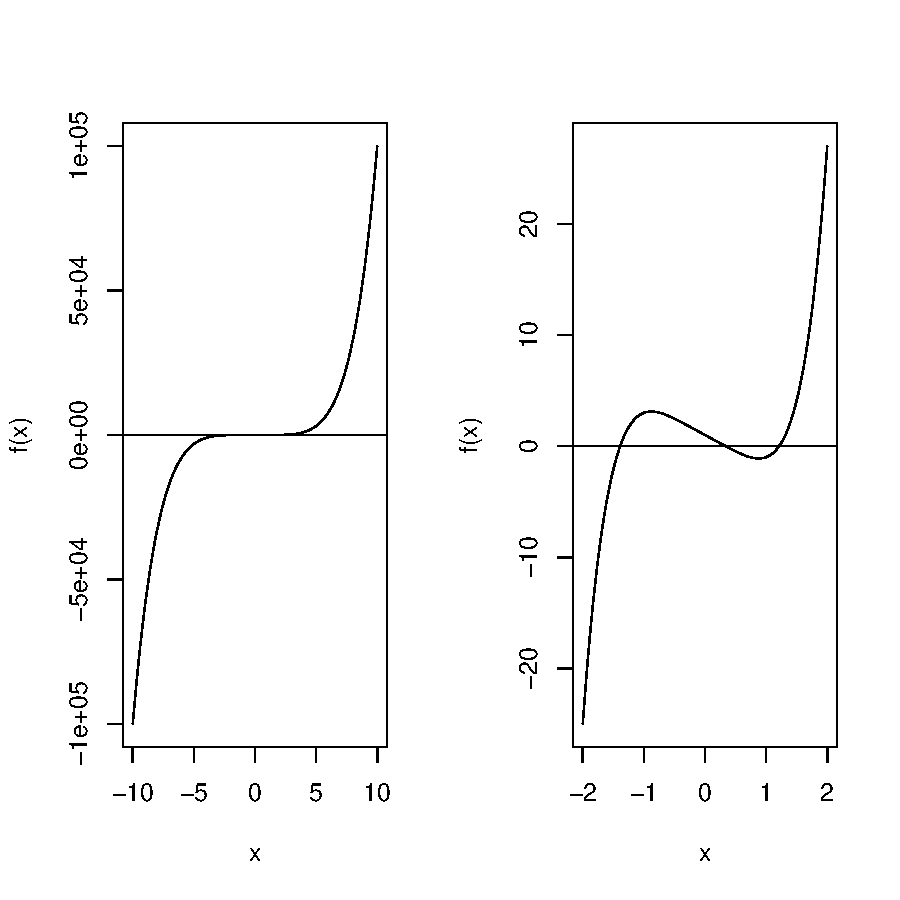
\includegraphics{Rmatematica-126}
\caption{Intersezione con l'asse $x$ }
\label{fig:newton}
\end{center}
\end{figure}

Dal grafico~\ref{fig:newton}  \`e evidente che ci sono 3 intersezioni con l'asse delle $x$ che ci proponiamo di determinare usando il metodo delle tangenti di Newton. Ricordiamo che nel metodo delle tangenti di Newton si deve scegliere un punto iniziale $x_0$  ed il numero di iterazioni (o un criterio di arresto).  Il passo iterativo \`e descritto dalla funzione:
$$g(x)=x-\frac{f(x)}{f'(x)}$$
In assenza della derivata esatta possiamo anche usare la regola dei 3 punti.
In quanto segue ipotizzeremo di avere scelto un 10 iterazioni a partire dal valore $x_0=2$.

\begin{Schunk}
\begin{Sinput}
> x<-2
\end{Sinput}
\end{Schunk}
Scegliamo un incremento
$h=10^{-3}$ ed 
iteriamo il processo attraverso un ciclo \texttt{for}\footnote{Il comando   \texttt{for(k in set) comando} esegue il \texttt{comando} (eventualmente dipendente da \texttt{k} per tutti i valori di \texttt{k} in \texttt{set}. }:

\begin{Schunk}
\begin{Sinput}
> h<-0.001
> for(k in 1:9) x[k+1]<-x[k]-f(x[k])/trepunti(f,x[k],h)
> x
\end{Sinput}
\begin{Soutput}
 [1] 2.000000 1.649351 1.406489 1.268587 1.220370
 [6] 1.214721 1.214648 1.214648 1.214648 1.214648
\end{Soutput}
\end{Schunk}
Si genera la lista di 10 passi iterativi, il fatto che la lista si stabilizzi \`e indice del fatto che la lista converge all'intersezione cercata.  Ricerchiamo anche un altro valore della {\it radice}:
\begin{Schunk}
\begin{Sinput}
> x<- -2; iterazioni=10;
> for(k in seq(length=iterazioni)) x[k+1]<-x[k]-f(x[k])/
+ trepunti(f,x[k],h)
> x
\end{Sinput}
\begin{Soutput}
 [1] -2.000000 -1.675325 -1.478238 -1.400446 -1.389020
 [6] -1.388792 -1.388792 -1.388792 -1.388792 -1.388792
[11] -1.388792
\end{Soutput}
\end{Schunk}
Per determinare la terza ed ultima intersezione partiamo da $x_0=0.5$
\begin{Schunk}
\begin{Sinput}
> x<-0.5
> for(k in 1:10) x[k+1]<-x[k]-
+ f(x[k])/trepunti(f,x[k],h);x
\end{Sinput}
\begin{Soutput}
 [1] 0.5000000 0.3255812 0.3347240 0.3347341 0.3347341
 [6] 0.3347341 0.3347341 0.3347341 0.3347341 0.3347341
[11] 0.3347341
\end{Soutput}
\end{Schunk}
Le radici sono 0.3347341, -1.388792, 1.214648.
\section{Integrali definiti}
Ci occupiamo ora del calcolo di integrali definiti
\begin{eqnarray*}
\int_a^b f(x)dx
\end{eqnarray*}

\subsection{Metodi numerici di integrazione di \textsf{R}}
Per il calcolo di integrali definiti si scrive il comando
\begin{eqnarray*}
\texttt{integrate}(\varia{funzione},
\varia{estremo inferiore}, \varia{estremo superiore})
\end{eqnarray*}
Ad esempio per $x$ tra -1 e 2
\begin{Schunk}
\begin{Sinput}
> integrate(function(x) x^4,-1,2) 
\end{Sinput}
\begin{Soutput}
6.6 with absolute error < 7.3e-14
\end{Soutput}
\end{Schunk}
Il risultato \`e un numero e di tale numero viene fornito l'errore assoluto, molto basso (la tecnica utilizzata \`e buona).
\subsection{Metodi di integrazione: metodo dei rettangoli e metodo dei trapezi}
Ci proponiamo di calcolare $$\int_a^b f(x)dx$$ suddividendo $[a,b]$ in $n$ sottointervalli di eguale ampiezza. Richiamiamo la procedura:  si suddivide l'intervallo $[a,b]$ in $n$ sottointervalli di egual ampiezza determinando il passo del metodo
$h=\dfrac{b-a}{n}$
e gli estremi degli intervalli 
$x_k=a+ k\, h$ con $k=0,\ldots,n$. Si calcolano poi i corrispondenti valori  $y_k=f(x_k)$ e si applicano poi le formule
\begin{eqnarray*}
L_n=h \sum_{i=0}^{n-1} y_k\\
R_n=h \sum_{i=1}^{n} y_k\\
T_n=\frac{L_n+R_n}{2}\end{eqnarray*}
che forniscono rispettivamente le stime a sinistra e a destra (metodo dei rettangoli) e la stima con il metodo dei trapezi.
Integriamo per esempio  una funzione $f(x)=x\, cos(x)$ con $n=10$, tra $a=1$ e $b=4$. Per prima cosa occorre determinare  il valore del passo.
\begin{Schunk}
\begin{Sinput}
> 10->n
> 1->a
> 4->b
> (b-a)/n->h
\end{Sinput}
\end{Schunk}
Con il comando   
\begin{Schunk}
\begin{Sinput}
> a+(0:n)*h->x;x
\end{Sinput}
\begin{Soutput}
 [1] 1.0 1.3 1.6 1.9 2.2 2.5 2.8 3.1 3.4 3.7 4.0
\end{Soutput}
\end{Schunk}
o anche con il comando
\begin{Schunk}
\begin{Sinput}
> x=seq(a,b,length=n+1)
\end{Sinput}
\end{Schunk}
si ottengono gli estremi degli intervalli. Si calcolano poi i valori corrispondenti della funzione e li si sostituiscono nelle formule di approssimazione
\begin{Schunk}
\begin{Sinput}
> f<-function(x) cos(x)*x
> f(x)
\end{Sinput}
\begin{Soutput}
 [1]  0.54030231  0.34774848 -0.04671924 -0.61425018
 [5] -1.29470246 -2.00285904 -2.63822255 -3.09731897
 [9] -3.28711385 -3.13797012 -2.61457448
\end{Soutput}
\begin{Sinput}
> y<-f(x)
> ln<-h*sum(y[1:n] )
> rn<-h*sum(y[2:(n+1)])
> tn<-(ln+rn)/2
> tn
\end{Sinput}
\begin{Soutput}
[1] -5.042563
\end{Soutput}
\end{Schunk}
Il confronto con il valore dell'integrale
\begin{Schunk}
\begin{Sinput}
> integrate(f,1,4)
\end{Sinput}
\begin{Soutput}
-5.062627 with absolute error < 6e-14
\end{Soutput}
\end{Schunk}
\`e abbastanza buono. Aumentando il numero di punti della suddivisione la stima migliora.
\begin{Schunk}
\begin{Sinput}
> 100->n
> (b-a)/n->h
> seq(a,b,length=(n+1))->x
> y<-f(x)
> ln<-h*sum(y[1:n])
> rn<-h*sum(y[2:(n+1)])
> tn<-(ln+rn)/2
> tn
\end{Sinput}
\begin{Soutput}
[1] -5.062426
\end{Soutput}
\begin{Sinput}
> rn
\end{Sinput}
\begin{Soutput}
[1] -5.109749
\end{Soutput}
\begin{Sinput}
> ln
\end{Sinput}
\begin{Soutput}
[1] -5.015103
\end{Soutput}
\end{Schunk}
  
\subsection{Metodo Montecarlo}
Supponiamo di voler applicare il metodo Montecarlo alla determinazione dell'integrale
\begin{equation*}
\int_1^4{ (x^3+3x)dx}
\end{equation*}
\begin{figure}[htbp]
\begin{center}
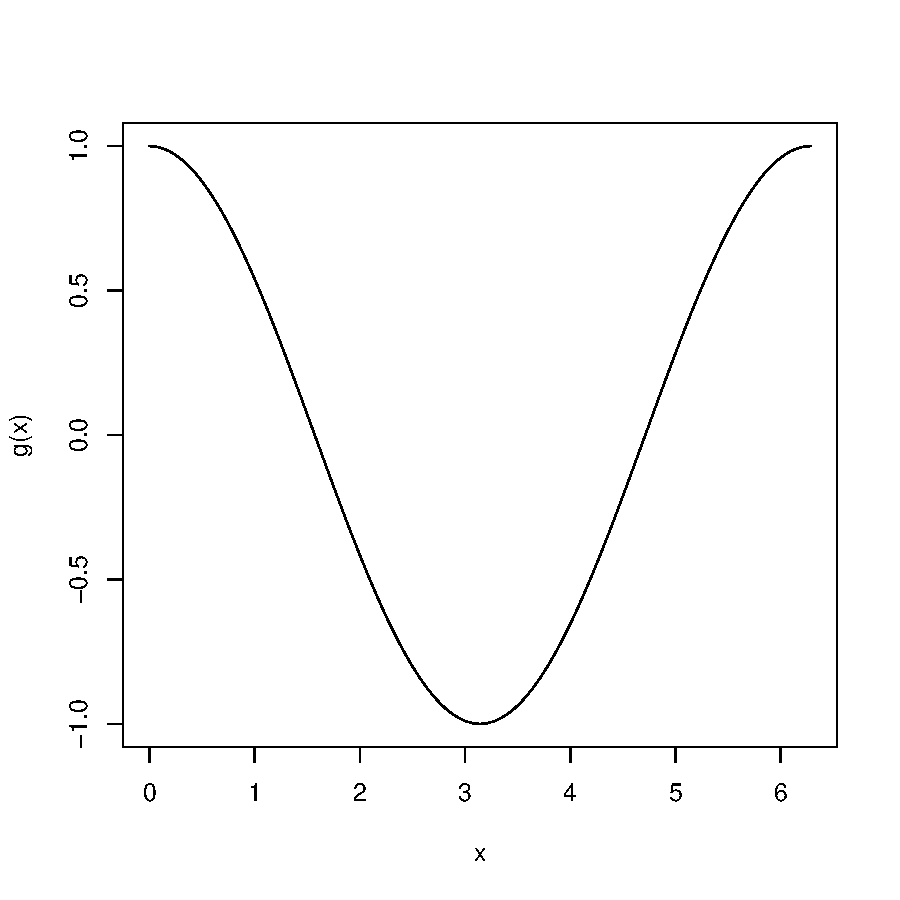
\includegraphics{Rmatematica-138}
\caption{Determinazione del bersaglio }
\label{fig:dgefault}
\end{center}
\end{figure}

Occorre determinare la finestra grafica da utilizzare come bersaglio. Nell'esempio $x$ varia tra 1 e 4. 
Per quanto riguarda la  $y$  tracciamo il grafico della funzione 

\begin{Schunk}
\begin{Sinput}
> curve(x^3+3*x,1,4)
\end{Sinput}
\end{Schunk}
Questa \`e una funzione crescente (fatto che avrei potuto determinare anche dallo studio del segno della derivata) e nell'intervallo in esame ha un minimo  in $x=1$ e un massimo in $x=4$. I corrispondenti valori sono $m=4$ e $M=76$.
\begin{Schunk}
\begin{Sinput}
> f<-function(x) x^3+3*x
> f(4)
\end{Sinput}
\begin{Soutput}
[1] 76
\end{Soutput}
\begin{Sinput}
> f(1)
\end{Sinput}
\begin{Soutput}
[1] 4
\end{Soutput}
\end{Schunk}


Possiamo quindi definire il bersaglio come
$$[1,4]\times [0,76]$$
Dobbiamo definire il numero di tiri. 
Il comando $\texttt{runif}(n,a,b)$, ({\it r}andom-{\it unif}orm), permette di generare $n$ numeri nell'intervallo $(a,b)$ distribuiti uniformemente. Se l'intervallo non \`e specificato i numeri appartengono all'intervallo $(0,1)$.
Useremo il comando  \texttt{runif} per effettuare i tiri.

\par
\begin{Schunk}
\begin{Sinput}
> 1000->tiri;
> x<-runif(tiri,1,4)		 
> y<-runif(tiri,0,76)
> centri<-which(y<f(x))	 
> successi<-length(centri)
> successi/tiri*76*3                    
\end{Sinput}
\begin{Soutput}
[1] 83.22
\end{Soutput}
\begin{Sinput}
> integrate(f,1,4)
\end{Sinput}
\begin{Soutput}
86.25 with absolute error < 9.6e-13
\end{Soutput}
\begin{Sinput}
> plot(x[centri],y[centri],
+ col="red",cex=0.3)   
> points(x[-centri],y[-centri],
+ col="blue",cex=0.3)  
> curve(f,add=T)		
\end{Sinput}
\end{Schunk}
\begin{figure}[htbp]
\begin{center}
\begin{Schunk}
\begin{Soutput}
[1] 80.712
\end{Soutput}
\begin{Soutput}
86.25 with absolute error < 9.6e-13
\end{Soutput}
\end{Schunk}
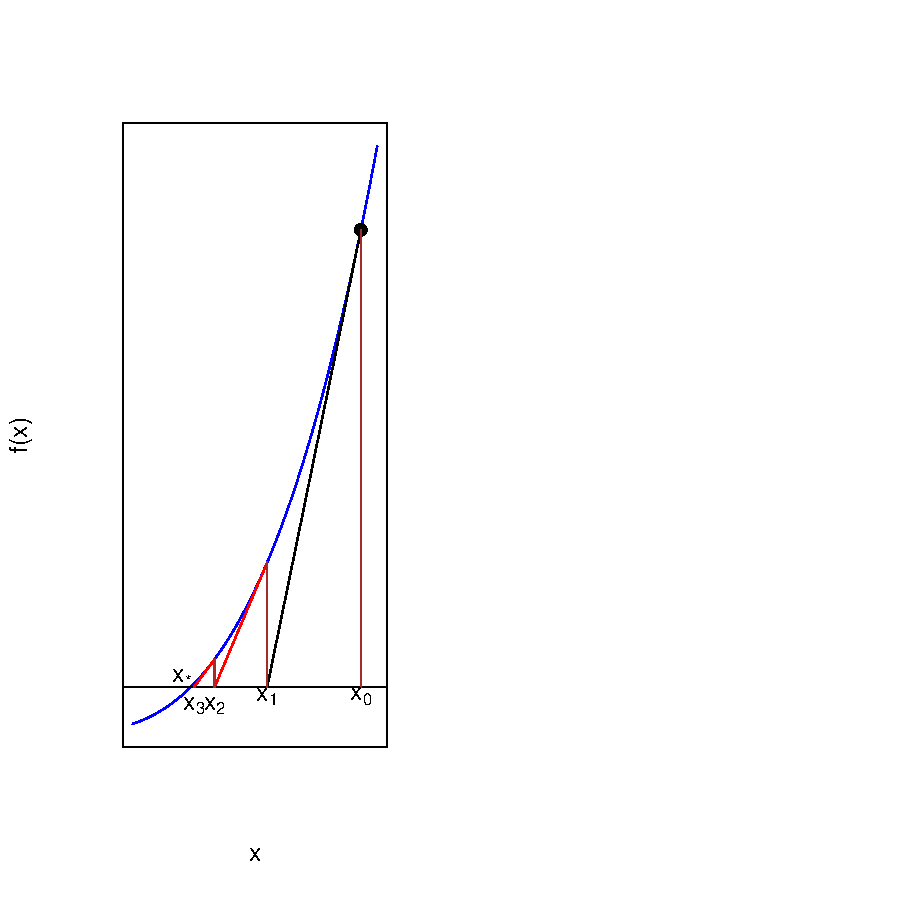
\includegraphics{Rmatematica-142}
\caption{Metodo Montecarlo }
\label{fig:Montec1}
\end{center}
\end{figure}
\end{document}
In modo simile possiamo considerare la determinazione di $\pi$. Immaginiamo di dover determinare l'area del cerchio di raggio 1 che \`e racchiuso nel quadrato $[-1,1]]\times[-1,1]$ del piano cartesiano.
In tal caso i comandi sono
\begin{Schunk}
\begin{Sinput}
> 10000->tiri;
> x<-runif(tiri,-1,1)		 
> y<-runif(tiri,-1,1)
> centri<-which(x^2+y^2<1)	 
> successi<-length(centri)
> successi/tiri*4                    
> plot(x[centri],y[centri],col="red",cex=0.4)   
> points(x[-centri],y[-centri], col="blue",cex=0.4)  
\end{Sinput}
\end{Schunk}

\begin{figure}[htbp]
\begin{center}
\begin{Schunk}
\begin{Soutput}
[1] 3.1268
\end{Soutput}
\end{Schunk}
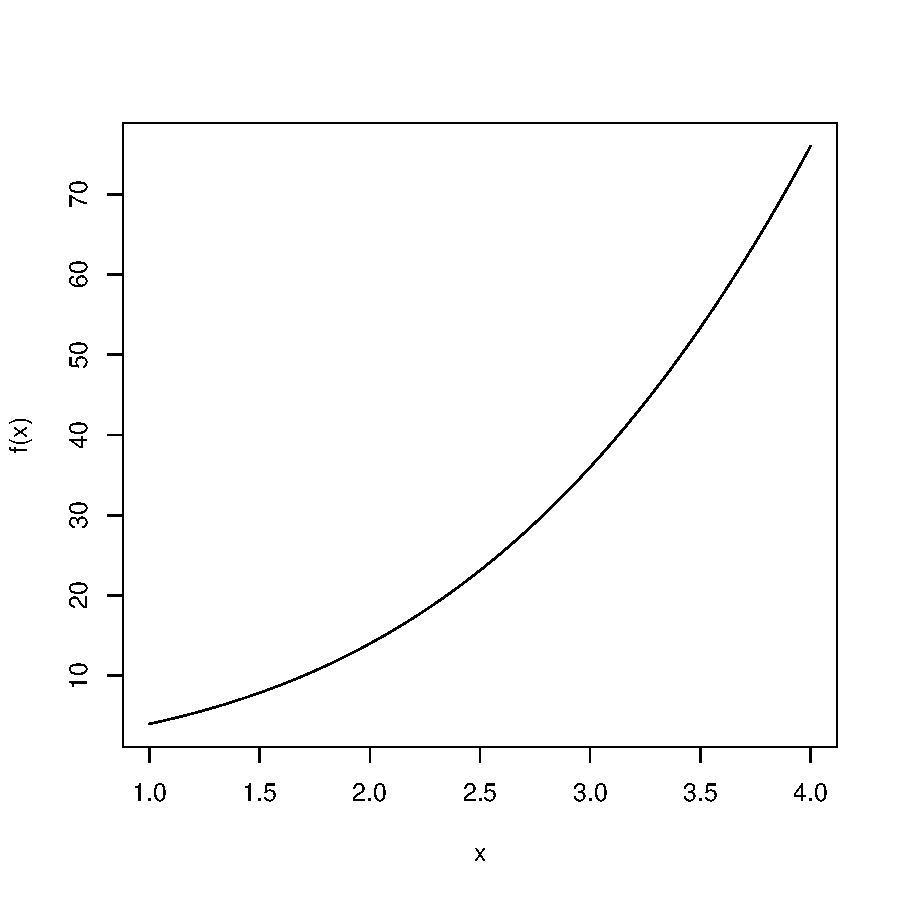
\includegraphics{Rmatematica-144}
\caption{Metodo Montecarlo per il disco}
\label{fig:newton}
\end{center}
\end{figure}
 SI noti che per ridurre la dimensione dei punti abbiamo usato l'opzione \texttt{cex}.
\section{Numeri complessi}
Un numero complesso viene indicato come $$z=a +ib$$ dove $a$  \`e la parte reale del numero complesso e $b$ il coefficiente della parte immaginaria $ib$.
In \textsf{R} un numero complesso viene scritto come
\begin{Schunk}
\begin{Sinput}
> z<-3 +4i
\end{Sinput}
\end{Schunk}
La componente immaginaria di un numero complesso contiene la lettera \texttt{\i} minuscola.  \`E possibile effettuare somme, sottrazioni, moltiplicazioni e divisioni usando i soliti simboli
\begin{Schunk}
\begin{Sinput}
> 2i+(4+5i)
\end{Sinput}
\begin{Soutput}
[1] 4+7i
\end{Soutput}
\begin{Sinput}
> (3+2i)*(3-1i)
\end{Sinput}
\begin{Soutput}
[1] 11+3i
\end{Soutput}
\begin{Sinput}
> (3+5i)/(4+2i)
\end{Sinput}
\begin{Soutput}
[1] 1.1+0.7i
\end{Soutput}
\end{Schunk}
 Alcune semplici operazioni con i numeri complessi
\begin{itemize}
\item{} La parte reale del numero complesso \varia{z} si indica con \texttt{Re}(\varia{z})
\begin{Schunk}
\begin{Sinput}
> z<-3+4i
> Re(z)
\end{Sinput}
\begin{Soutput}
[1] 3
\end{Soutput}
\end{Schunk}

\item{} Il coefficiente della parte immaginaria di \varia{z} si indica con
 \texttt{Im}(\varia{z})
\begin{Schunk}
\begin{Sinput}
>  Im(z)
\end{Sinput}
\begin{Soutput}
[1] 4
\end{Soutput}
\end{Schunk}
\item{}Il coniugato del numero complesso $z=a +ib$ \`e $\overline{z}=a-ib$. In \textsf{R} si usa la funzione \text{Conj}:

\begin{Schunk}
\begin{Sinput}
> Conj(z)
\end{Sinput}
\begin{Soutput}
[1] 3-4i
\end{Soutput}
\end{Schunk}
\item{}L'argomento \texttt{arg} di un numero complesso $z=a +i b$ \`e definito come 
$\texttt{arg}(z) =\texttt{arctan}(b/a)$. In  \textsf{R} si usa
\texttt{Arg}(\varia{z})
e per esempio
\begin{Schunk}
\begin{Sinput}
>  Arg(z)
\end{Sinput}
\begin{Soutput}
[1] 0.9272952
\end{Soutput}
\begin{Sinput}
> atan(4/3)
\end{Sinput}
\begin{Soutput}
[1] 0.9272952
\end{Soutput}
\end{Schunk}
\item{}Il modulo di  un numero complesso \`e semplicemente $\sqrt(z*\overline{z})$ ed \`e indicato in \textsf{R} con  \text{Mod}(\varia{z})
\begin{Schunk}
\begin{Sinput}
> Mod(z)
\end{Sinput}
\begin{Soutput}
[1] 5
\end{Soutput}
\end{Schunk}
\item{}L'esponenziale con esponente complesso si indica come al solito con
\texttt{exp}(\varia{z}) 
\begin{Schunk}
\begin{Sinput}
> exp(z)
\end{Sinput}
\begin{Soutput}
[1] -13.12878-15.20078i
\end{Soutput}
\begin{Sinput}
> exp(z)*exp(Conj(z))   		
\end{Sinput}
\begin{Soutput}
[1] 403.4288+0i
\end{Soutput}
\end{Schunk}
\end{itemize}
